\documentclass[11pt,letterpaper]{article}

%% ── Packages ──────────────────────────────────────────────────────────────────
\usepackage[margin=1in]{geometry}
\usepackage{amsmath}
\usepackage{amssymb}
\usepackage{booktabs}
\usepackage{graphicx}
\usepackage{float}
\usepackage{siunitx}
\usepackage{hyperref}
\usepackage{xcolor}
\usepackage{enumitem}
\usepackage{array}
\usepackage{caption}
\usepackage{parskip}

%% ── Document metadata ─────────────────────────────────────────────────────────
\title{\textbf{MEEN 305 Final Project}\\[0.5em]
       \large Minimum-Weight Beam Design and Analysis\\[0.3em]
       \large Tapered Hollow Rectangular Tube in PLA}
\author{Team \#6}
\date{Spring 2026}

\setcounter{tocdepth}{2}

\begin{document}
\maketitle
\tableofcontents
\newpage

%% ═══════════════════════════════════════════════════════════════════════════════
\section{Problem Statement and Requirements}
%% ═══════════════════════════════════════════════════════════════════════════════

\subsection{Fixed Project Inputs}

The beam is simply supported with the following prescribed boundary conditions
and loading:

\begin{center}
\begin{tabular}{lll}
\toprule
Parameter & Symbol & Value \\
\midrule
Support span & $L$ & \SI{8.0}{in} \\
Total beam length & $L_{total}$ & \SI{9.0}{in} \\
Load Case~1 magnitude & $P_1$ & \SI{5.0}{lbf} \\
Load Case~1 location & $a_1$ & \SI{4.0}{in} from support~A (midspan) \\
Load Case~1 orientation & N/A & Upright (load applied vertically) \\
Load Case~2 magnitude & $P_2$ & \SI{8.0}{lbf} \quad ($2 + \text{Team\#} = 2 + 6$) \\
Load Case~2 location & $a_2$ & \SI{5.0}{in} from support~A \quad ($2 + \tfrac{6}{2} = 5$) \\
Load Case~2 orientation & N/A & Rotated \SI{90}{\degree} about span axis \\
Required factor of safety & $\mathrm{FoS}_{\min}$ & $\ge 1.5$ for both load cases \\
\bottomrule
\end{tabular}
\end{center}

\subsection{Objective}

Minimize the weight of the printed beam,
\[
  \text{minimize}\quad W = \rho \int_0^{L} A(x)\,dx,
\]
subject to the factor-of-safety constraint for both load cases and all
engineering and manufacturing constraints defined in Section~\ref{sec:constraints}.

\subsection{Design Variables}

The beam cross-section is a tapered hollow rectangular tube with spanwise
lightening openings.  The geometry is fully described by \textbf{10 continuous
design variables}:

\begin{center}
\begin{tabular}{llll}
\toprule
Variable & Symbol & Units & Role \\
\midrule
Left/mid/right outer width   & $b_L, b_M, b_R$ & in & Tube width at $x=0,L/2,L$ \\
Left/mid/right outer height  & $h_L, h_M, h_R$ & in & Tube height at $x=0,L/2,L$ \\
Wall thickness               & $t$             & in & Uniform flange/web thickness \\
Left/mid/right opening ratio & $r_L, r_M, r_R$ & -- & Fraction of inner web height removed \\
\bottomrule
\end{tabular}
\end{center}

All six profile dimensions ($b$, $h$, $r$) vary continuously along the span
via piecewise linear interpolation between the three control points.  Wall
thickness $t$ is kept spatially uniform, consistent with FDM slice practice.


%% ═══════════════════════════════════════════════════════════════════════════════
\section{Material Selection}
\label{sec:material}
%% ═══════════════════════════════════════════════════════════════════════════════

\subsection{Available FDM Polymers}

The Rapid Prototyping Studio (JCAIN 422) stocks four filament options.
Their nominal bulk properties and effective FDM properties are:

\begin{center}
\begin{tabular}{lrrrrrr}
\toprule
Material & $E$ [psi] & $\sigma_{allow}$ [psi] & $\rho$ [\si{lbf/in^3}]
         & $k_{orient}$ & $k_{infill}$ & $E_{eff}$ [psi] \\
\midrule
PLA  & 500\,000 & 4\,000 & 0.045 & 0.70 & 0.85 & 297\,500 \\
ASA  & 380\,000 & 3\,600 & 0.043 & 0.65 & 0.85 & 209\,950 \\
PETG & 290\,000 & 3\,500 & 0.046 & 0.72 & 0.85 & 177\,480 \\
TPU  &  10\,000 & 2\,500 & 0.043 & 0.75 & 0.90 &   6\,750 \\
\bottomrule
\end{tabular}
\end{center}

\subsection{Orientation and Infill Factors}

FDM parts are mechanically anisotropic because deposited layers bond through
partial re-melting.  The interlayer bond is the dominant failure surface.
Two reduction factors are applied multiplicatively to all nominal isotropic
properties:

\begin{itemize}[noitemsep]
  \item \textbf{Orientation factor} $k_{orient}$: accounts for the reduction
    in strength and stiffness perpendicular to the print plane.  When the span
    axis lies along the print direction (layer lines parallel to the neutral
    axis), load is transferred through the solid infill struts rather than
    across layer interfaces.  We use $k_{orient} = 0.70$ for PLA, consistent
    with RPS guidance that layer lines are ``the single biggest failure point.''
  \item \textbf{Infill factor} $k_{infill}$: accounts for the reduced
    solid volume at less-than-100\% rectilinear infill.  We use
    $k_{infill} = 0.85$, corresponding to approximately 40\% rectilinear
    infill with solid top/bottom shells.  The physical beams were actually
    printed at 100\% infill density (confirmed from the slicer project file),
    making the fabricated parts stiffer and stronger than the model predicts.
    This means measured deflections may be somewhat lower than the theoretical
    values, and the actual factor of safety exceeds the computed minimum.
\end{itemize}

Effective properties:
\[
  E_{eff} = k_{orient}\,k_{infill}\,E_{bulk}
  = 0.70 \times 0.85 \times 500\,000 = 297\,500\ \mathrm{psi}
\]
\[
  \sigma_{allow,eff} = k_{orient}\,k_{infill}\,\sigma_{allow}
  = 0.70 \times 0.85 \times 4\,000 = 2\,380\ \mathrm{psi}
\]

\subsection{Justification for PLA}

PLA is selected for the following engineering reasons:

\begin{enumerate}[noitemsep]
  \item \textbf{Highest effective stiffness}: $E_{eff,PLA} = 297\,500$ psi
    versus $209\,950$, $177\,480$, and $6\,750$ psi for ASA, PETG, and TPU
    respectively.  Deflection is inversely proportional to $E_{eff}I$;
    PLA permits the smallest cross-section for a given deflection.
  \item \textbf{Highest allowable stress}: $\sigma_{allow,eff,PLA} = 2\,380$
    psi gives the largest FoS margin for a given cross-section, enabling
    more material removal.
  \item \textbf{Printability}: PLA is the recommended default at the RPS and
    requires no special enclosure or bed adhesion, making reliable prints
    more likely.
  \item \textbf{Density}: PLA density ($0.045\ \mathrm{lbf/in^3}$) is
    representative of structural polymers; ASA is marginally lighter but
    at the cost of significantly lower effective properties.
\end{enumerate}

TPU is immediately eliminated (flexible elastomer, not a structural polymer).
ASA and PETG are eliminated because both have lower $E_{eff}$ and lower
$\sigma_{allow,eff}$ than PLA; the same geometry would be heavier and weaker.


%% ═══════════════════════════════════════════════════════════════════════════════
\section{Beam Parametrization}
\label{sec:parametrization}
%% ═══════════════════════════════════════════════════════════════════════════════

\subsection{Cross-Section Topology}

At each spanwise location $x$, the cross-section is a hollow rectangular tube
with a centered web opening (lightening slot) in both vertical web faces.
The outer dimensions at position $x$ are $b(x) \times h(x)$; the wall
thickness $t$ is uniform throughout.  The opening removes a fraction $r(x)$
of the clear inner web height $h_{clear}(x) = h(x) - 2t$ from both web faces,
leaving solid flanges top and bottom.

\subsection{Profile Functions}

Each of the three continuous profiles is defined by piecewise linear
interpolation between three control points at $x = 0$ (left support),
$x = L/2 = 4\ \mathrm{in}$ (midspan), and $x = L = 8\ \mathrm{in}$
(right support):

\[
  b(x) = \begin{cases}
    b_L + \dfrac{2(b_M - b_L)}{L}\,x, & 0 \le x \le \tfrac{L}{2} \\[6pt]
    b_M + \dfrac{2(b_R - b_M)}{L}\,(x - \tfrac{L}{2}), & \tfrac{L}{2} < x \le L
  \end{cases}
\]

and analogously for $h(x)$ and $r(x)$.  This three-point piecewise-linear
scheme provides enough shape freedom to represent arch profiles, linearly
tapered beams, and uniform beams as special cases, while keeping the number
of design variables tractable.

\subsection{Section Properties}

\paragraph{Cross-sectional area (with openings).}
\[
  A(x) = 2\,b(x)\,t + [1 - r(x)]\,2\,t\,h_{clear}(x),
  \quad h_{clear}(x) = h(x) - 2t
\]
The first term is the two horizontal flanges; the second is the remaining
vertical web area after the lightening slot is removed.

\paragraph{Second moment of area: upright bending (Load Case~1).}
The full hollow-tube second moment minus the two opening slots:
\[
  I_{upright}(x) = \frac{b(x)\,h(x)^3 - [b(x)-2t]\,[h(x)-2t]^3}{12}
  - 2\,\frac{t\,[r(x)\,(h(x)-2t)]^3}{12}
\]

\paragraph{Second moment of area: side-rotated bending (Load Case~2).}
The beam is physically rotated \SI{90}{\degree} about the span axis, so $b$
becomes the vertical (bending) dimension and $h$ becomes the lateral dimension:
\[
  I_{side}(x) = \frac{h(x)\,b(x)^3 - [h(x)-2t]\,[b(x)-2t]^3}{12}
  - 2\,\frac{t\,[r(x)\,(b(x)-2t)]^3}{12}
\]

\paragraph{Section modulus.}
The section modulus uses $c_y(x)$ for upright bending (extreme fiber in the
$y$-direction, i.e.\ half the outer height) and $c_z(x)$ for side-rotated
bending (extreme fiber in the $z$-direction, i.e.\ half the outer width):
\[
  S_{upright}(x) = \frac{I_{upright}(x)}{c_y(x)},
  \qquad c_y(x) = \frac{h(x)}{2}
\]
\[
  S_{side}(x) = \frac{I_{side}(x)}{c_z(x)},
  \qquad c_z(x) = \frac{b(x)}{2}
\]

\paragraph{Shear area.}
\[
  A_{shear}(x) = [1 - r(x)]\,2t\,h_{clear,active}(x)
\]
where $h_{clear,active}$ is the clear inner dimension in the active bending
orientation: $h_{clear}(x) = h(x)-2t$ for upright, $(b(x)-2t)$ for side.

\begin{figure}[H]
  \centering
  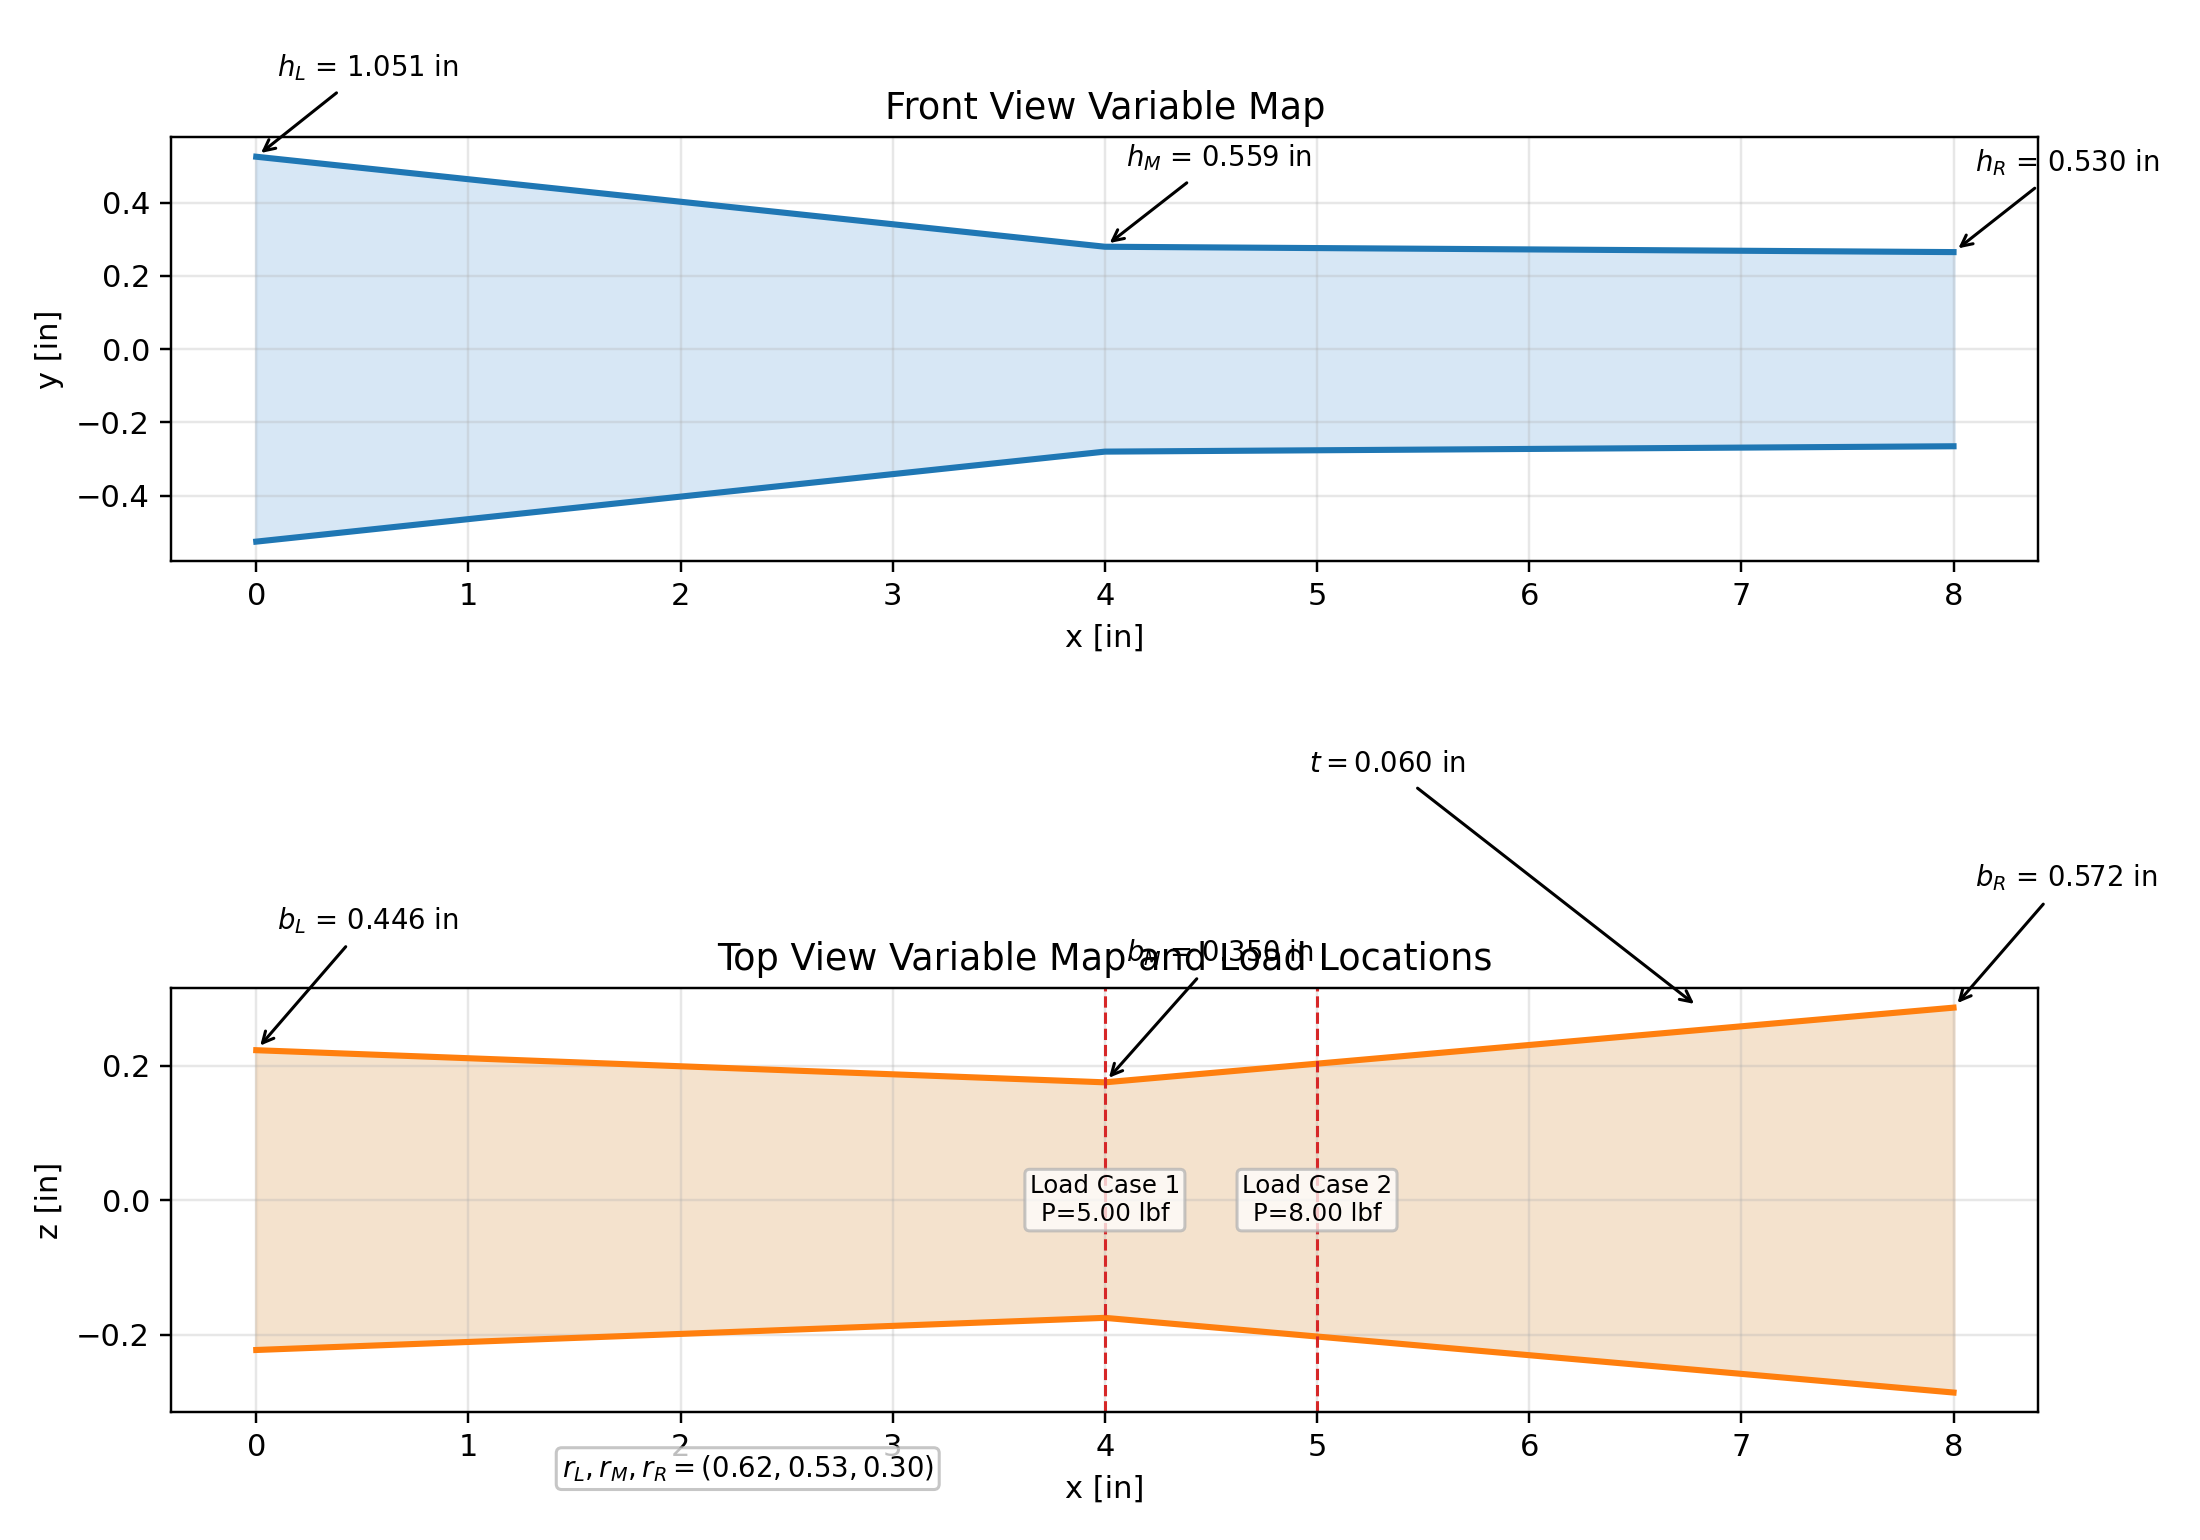
\includegraphics[width=0.85\textwidth]{../../archive/deprecated_assets/optimization_final/beam_parameter_map.png}
  \caption{Variable map for the final optimized design.  Front view (top) shows
  the height profile $h(x)$ with control-point annotations; top view (bottom)
  shows the width profile $b(x)$, wall thickness $t$, and load locations.}
  \label{fig:parammap}
\end{figure}

\begin{figure}[H]
  \centering
  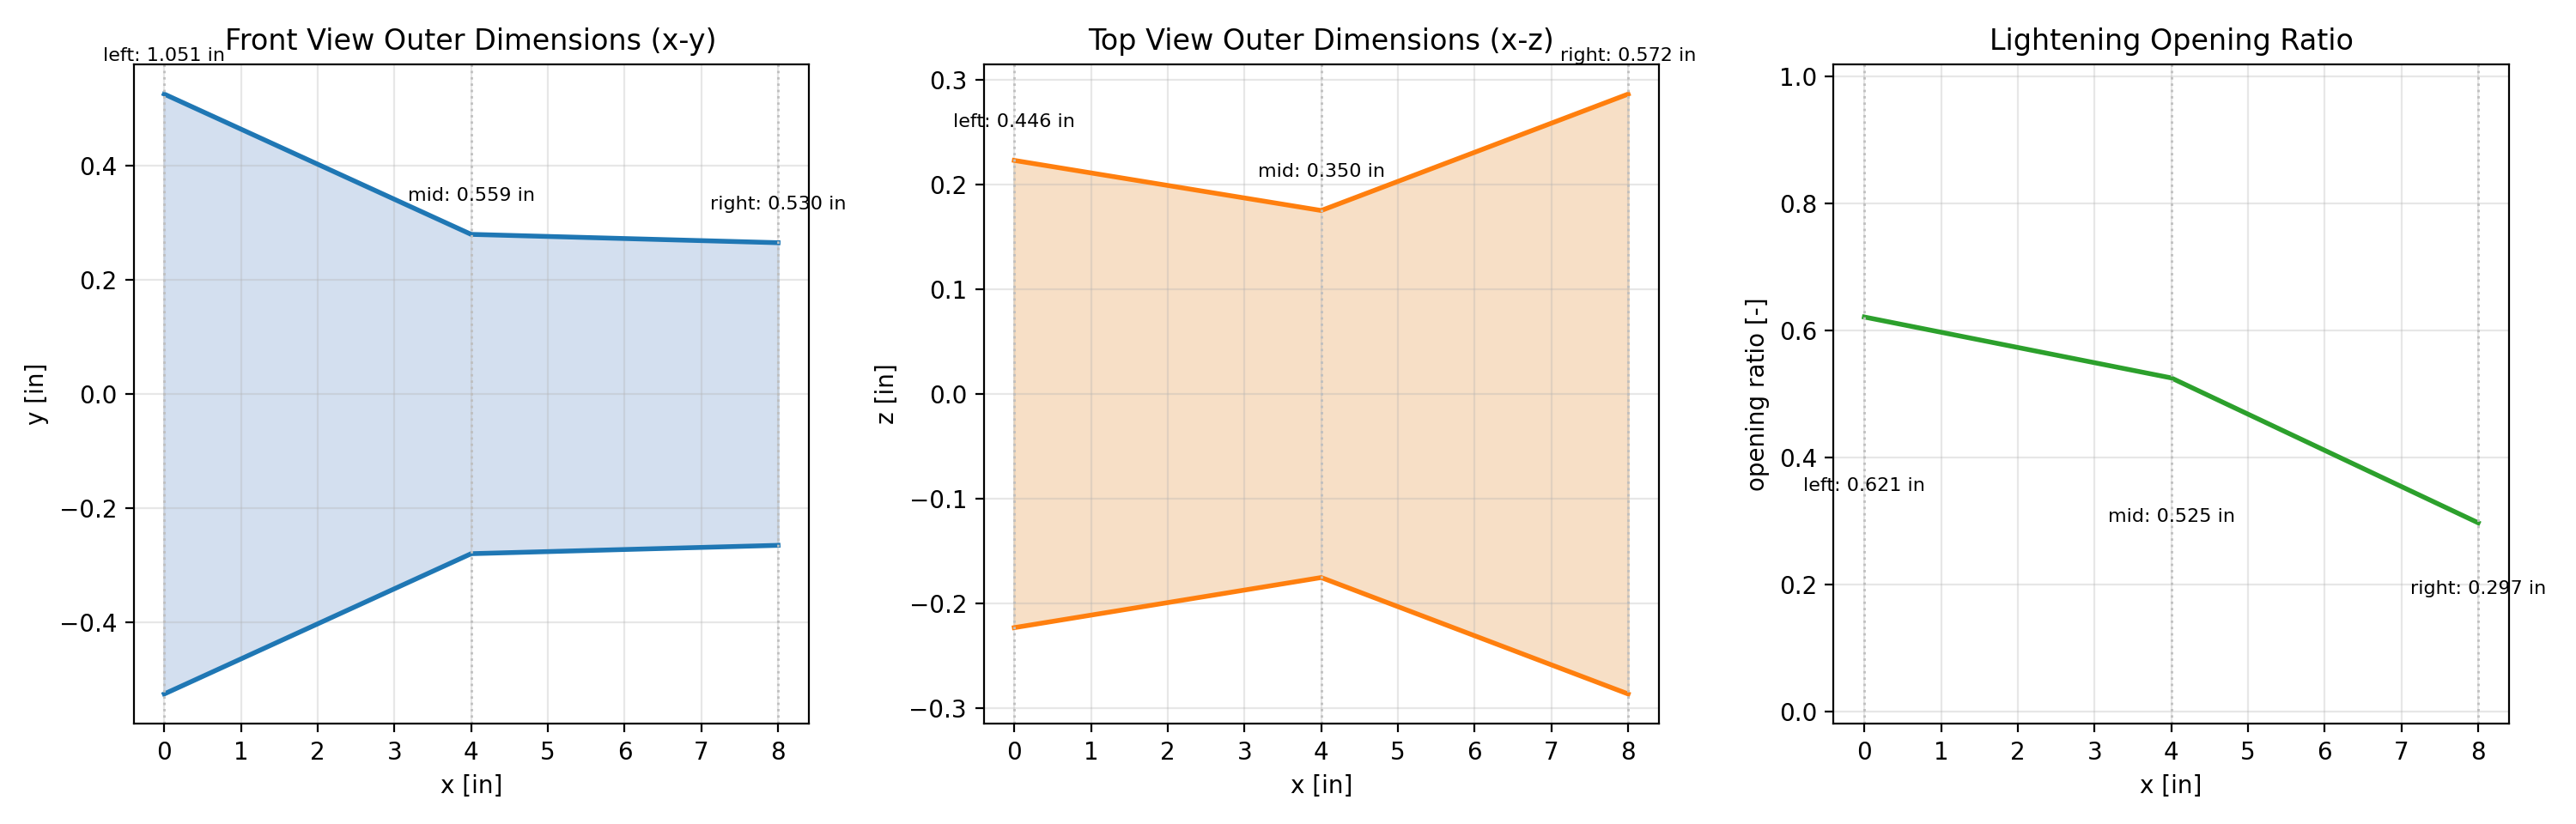
\includegraphics[width=\textwidth]{../../archive/deprecated_assets/optimization_final/best_design/outer_dimension_views.png}
  \caption{Outer dimension profiles and lightening-opening ratio for the
  final design.  Left: front-view height profile $h(x)$; centre: top-view
  width profile $b(x)$; right: web opening ratio $r(x)$ along the span.}
  \label{fig:outerviews}
\end{figure}


%% ═══════════════════════════════════════════════════════════════════════════════
\section{Governing Equations and Analysis Methodology}
\label{sec:theory}
%% ═══════════════════════════════════════════════════════════════════════════════

\subsection{Statics: Reactions and Internal Loads}

For a simply supported beam with one point load $P$ at $x = a$:
\[
  R_A = \frac{P(L-a)}{L}, \qquad R_B = \frac{Pa}{L}
\]

Shear force and bending moment (piecewise, with the load-point discontinuity):
\[
  V(x) = \begin{cases} R_A & 0 \le x < a \\ R_A - P & a < x \le L \end{cases}
  \qquad
  M(x) = \begin{cases} R_A\,x & 0 \le x < a \\ R_A\,x - P(x-a) & a < x \le L \end{cases}
\]

\subsection{von Mises Stress}

The von Mises criterion combines all stress components into one scalar that
can be compared directly against the effective allowable stress.  The three
intermediate quantities that feed into it are:

\paragraph{Normal bending stress.}
Using the Euler-Bernoulli flexure formula at the extreme fiber
(distance $c_y$ or $c_z$ from the neutral axis, depending on orientation):
\[
  \sigma_b(x) = \frac{|M(x)|}{S(x)}
\]

\paragraph{Shear stress.}
Shear is distributed over the active web area remaining after the lightening
opening.  A conservative uniform-distribution approximation is used:
\[
  \tau(x) = \frac{|V(x)|}{A_{shear}(x)}
\]

\paragraph{von Mises equivalent stress.}
For the plane-stress state at the critical point (bending-dominant at the
extreme fiber, shear-dominant at the neutral axis):
\[
  \sigma_{vm}(x) = \sqrt{\sigma_b(x)^2 + 3\,\tau(x)^2}
\]

The $\sigma_b^2$ term dominates wherever $|M(x)|$ is large (e.g.\ midspan);
the $3\tau^2$ term dominates near the supports where $M \to 0$ but $V$ is
nonzero.  The governing (maximum) von Mises stress determines the minimum
FoS over the span.

\subsection{Factor of Safety}

\[
  \mathrm{FoS}(x) = \frac{\sigma_{allow,eff}}{\sigma_{vm}(x)}
\]

The governing (minimum) FoS is tracked at every discretized station $x$
across both load cases:
\[
  \mathrm{FoS}_{min} = \min_{x,\,\text{LC}} \mathrm{FoS}(x)
\]

The design constraint is $\mathrm{FoS}_{min} \ge 1.5$.

\subsection{Deflection via Euler-Bernoulli Integration}

The Euler-Bernoulli beam equation for a non-uniform cross-section:
\[
  E_{eff}\,I(x)\,v''(x) = M(x)
\]

Because $I(x)$ varies continuously with $x$, slope $\theta(x) = v'(x)$
and deflection $v(x)$ are obtained by numerical integration (trapezoidal rule,
801 stations) with simple-support boundary conditions $v(0) = v(L) = 0$:

\begin{align*}
  \theta(x) &= \int_0^x \frac{M(s)}{E_{eff}\,I(s)}\,ds + C_1 \\
  v(x) &= \int_0^x \theta(s)\,ds + C_1\,x
\end{align*}

The integration constant $C_1$ is determined by enforcing $v(L) = 0$.

\subsection{Beam Weight}

\[
  W = \rho \int_0^{L} A(x)\,dx
\]

The integral is evaluated numerically over the same 801-station grid.

\subsection{Assumption: Self-Weight Neglected}

\textbf{Self-weight is not included in the shear, moment, stress, or
deflection calculations.}  Justification:

\begin{itemize}[noitemsep]
  \item The optimized beam weighs $W = 0.03454\ \mathrm{lbf}$.
  \item Applied point loads total $P_1 + P_2 = 5 + 8 = 13\ \mathrm{lbf}$.
  \item Self-weight is $0.03454 / 13 \approx 0.27\%$ of applied load.
  \item Standard practice neglects distributed self-weight when it is less
    than 5\% of applied load.  At 0.27\%, the assumption is conservative
    by more than an order of magnitude; including self-weight would increase
    midspan stress by $< 0.3\%$.
\end{itemize}

\subsection{Equation Dependency Chain}

The full analysis pipeline from inputs to objective is:
\[
  (L,\,P,\,a)
  \;\xrightarrow{\text{statics}}\;
  R_A,\,R_B
  \;\xrightarrow{}\;
  V(x),\,M(x)
  \;\xrightarrow{\text{geometry}}\;
  A(x),\,I(x),\,S(x)
  \;\xrightarrow{}\;
  \sigma_b,\,\tau
  \;\xrightarrow{}\;
  \sigma_{vm}
  \;\xrightarrow{}\;
  \mathrm{FoS}
\]
\[
  M(x),\,E_{eff},\,I(x)
  \;\xrightarrow{\text{integration}}\;
  v(x)
  \qquad\qquad
  A(x),\,\rho
  \;\xrightarrow{\text{integration}}\;
  W
\]

Both load cases use the same geometry functions; the active bending
orientation switches between $I_{upright},\,c_y$ (LC1) and $I_{side},\,c_z$ (LC2).


%% ═══════════════════════════════════════════════════════════════════════════════
\section{Engineering Judgment Constraints}
\label{sec:constraints}
%% ═══════════════════════════════════════════════════════════════════════════════

An idealized stress analysis would permit geometries that are physically
unrealizable on an FDM printer.  The following engineering judgment constraints
are hard-coded in \texttt{beam\_solver.py} (\texttt{TaperedRectangularTube.validate()}):

\begin{enumerate}
  \item \textbf{Minimum cross-section at every station, including supports.}
    At a simply supported beam end, the bending moment is zero, so idealized
    theory requires zero section modulus (i.e., zero cross-section).  In
    reality, the beam must physically contact its supports and transfer shear.
    The code enforces $h(x), b(x) \ge 0.15\ \mathrm{in}$ ($\approx 3.8\ \mathrm{mm}$)
    at every station.

  \item \textbf{Minimum printable wall thickness.}
    A purely stress-based analysis would permit paper-thin walls wherever
    stress is low.  On a 0.4~mm nozzle, fewer than two continuous perimeters
    ($< 0.8\ \mathrm{mm}$) produces unreliable, porous walls.  The code
    enforces $t \ge 0.040\ \mathrm{in}$ ($\approx 1.0\ \mathrm{mm}$).

  \item \textbf{Wall thickness must fit inside the cross-section.}
    $t < b/2$ and $t < h/2$ at every station; otherwise the tube wall
    would overlap the centerline.

  \item \textbf{Ligament constraint for web openings.}
    The remaining solid ligament on each side of a web opening must exceed
    the wall thickness: $\tfrac{1}{2}(1 - r)\,h_{clear} > t$.  This ensures
    the web-to-flange junction is thick enough for load transfer and printing.

  \item \textbf{Opening ratio bounded below 0.95.}
    A ratio of 1.0 would remove the web entirely, leaving two unconnected
    flanges.  The code enforces $r < 0.95$.
\end{enumerate}

The \textbf{optimizer search bounds} are more restrictive than these hard
minimums, providing the primary engineering envelope:

\begin{center}
\begin{tabular}{lll}
\toprule
Variable & Optimizer minimum & Optimizer maximum \\
\midrule
Height $h$ [in]         & 0.38 & 1.30 \\
Width $b$ [in]          & 0.35 & 1.60 \\
Wall thickness $t$ [in] & 0.06 & 0.18 \\
Opening ratio $r$ [--]  & 0.00 & 0.87 \\
\bottomrule
\end{tabular}
\end{center}

The minimum height of $0.38\ \mathrm{in}$ ($\approx 9.7\ \mathrm{mm}$) ensures
a realistic cross-section at every station including at the supports.  The
maximum opening ratio of 0.87 was chosen to guarantee at least $1.9\ \mathrm{mm}$
of solid ligament per side at the minimum-height station, about 5 nozzle
widths at 0.4~mm, sufficient for a reliable continuous wall.


%% ═══════════════════════════════════════════════════════════════════════════════
\section{Optimization Methodology}
\label{sec:optimization}
%% ═══════════════════════════════════════════════════════════════════════════════

\subsection{Search Strategy}

A two-phase surrogate-free method was used:

\begin{enumerate}
  \item \textbf{Latin hypercube sampling (LHS).}
    600 candidate designs are drawn by stratified random sampling across the
    10-dimensional design space.  LHS guarantees that each variable's range
    is sampled uniformly, avoiding clustering inherent in purely random
    Monte Carlo sampling.

  \item \textbf{Elite local refinement.}
    After the global phase, the top 20 feasible designs (``elites'') are
    identified.  Around each elite, 35 new candidates are sampled from a
    Gaussian neighborhood with standard deviation shrinking by $1/(k+1)$
    each round.  This is repeated for 8 rounds, progressively concentrating
    the search near the current best design.
\end{enumerate}

Total designs evaluated: \textbf{1\,300}; feasible designs found: \textbf{684}.

\subsection{Objective Function}

The search minimizes a penalized composite objective:
\[
  f(\mathbf{d}) = W
  + 500\,\bigl(\max(0,\;1.5 - \mathrm{FoS}_{min})\bigr)^2
  + 12.0\,\bigl(\mathrm{FoS}_{min} - 1.5\bigr)^2
  + 0.5\,\overline{u}^2
\]

where:
\begin{itemize}[noitemsep]
  \item $W$ is beam weight [lbf], which is the true objective.
  \item The first penalty drives infeasible designs toward FoS $\ge 1.5$.
  \item The third term (weight 12.0) penalizes \emph{excess} FoS above 1.5;
    this is what drives the optimizer to remove material rather than
    stopping at the first feasible design.
  \item $\overline{u}^2$ is the mean-squared underutilization across beam
    stations, penalizing cross-sections far from the target stress level and
    encouraging a more uniform stress distribution.
\end{itemize}

The excess-FoS weight of 12.0 was determined through systematic trial.
Values below $\sim 1.0$ left the optimizer content with FoS $\gg 1.5$;
values above $\sim 20$ caused constraint violations.

\subsection{Why Load Case~2 Governs for Team~6}

For Team~6, $P_2 = 8\ \mathrm{lbf}$ at $a_2 = 5\ \mathrm{in}$
produces a maximum bending moment of:
\[
  M_{max,LC2} = R_{A,LC2} \times a_2
  = \frac{8(8-5)}{8} \times 5 = 3 \times 5 = 15\ \mathrm{lbf \cdot in}
\]

Load Case~1 produces:
\[
  M_{max,LC1} = R_{A,LC1} \times a_1
  = \frac{5(8-4)}{8} \times 4 = 2.5 \times 4 = 10\ \mathrm{lbf \cdot in}
\]

LC2 has 50\% more bending moment than LC1, and acts in the side-rotated
orientation where the width $b$ (not height $h$) is the critical bending
dimension.  This fundamentally changes the optimal design topology compared
to a team with a smaller $P_2$: the optimizer must now ensure adequate
\emph{width} at the location of peak LC2 moment.

\subsection{Printability Bounds}

Early runs produced designs with extreme height tapers
($h_{max}/h_{min} > 4\times$), which generated non-contiguous 3D meshes.
Capping the maximum height at $1.30\ \mathrm{in}$ limits the taper ratio
to $\le 2.13\times$ in the final design, ensuring a single contiguous
3D solid.


%% ═══════════════════════════════════════════════════════════════════════════════
\section{Final Optimized Design}
\label{sec:design}
%% ═══════════════════════════════════════════════════════════════════════════════

\subsection{Geometry}

\begin{center}
\begin{tabular}{lrl}
\toprule
Variable & Value & Notes \\
\midrule
$b_L$ [in] & 0.823 & Wide left end; carries LC2 side bending and LC1 shear \\
$b_M$ [in] & 0.350 & Minimum allowed; width is not the critical dimension at midspan \\
$b_R$ [in] & 0.350 & Minimum allowed; LC2 moment decreases toward right support \\
$h_L$ [in] & 0.959 & Tall left end provides LC1 upright bending capacity and web shear area \\
$h_M$ [in] & 0.727 & Moderate midspan height; LC1 upright bending governs here \\
$h_R$ [in] & 0.606 & Shorter right end; LC2 reaction is large at this support ($R_B=5$ lbf) \\
$t$ [in]   & 0.060 & Minimum allowed ($\approx 1.5\ \mathrm{mm}$, 3.75 nozzle widths) \\
$r_L$ [--] & 0.334 & 33\% web opening at left (limited by LC2 shear demand) \\
$r_M$ [--] & 0.650 & 65\% web opening at midspan where both moments are moderate \\
$r_R$ [--] & 0.276 & 28\% web opening at right where $R_B$ is largest \\
\bottomrule
\end{tabular}
\end{center}

\paragraph{Topology.}
The optimizer found a \textbf{left-heavy taper}: the left end is the widest
($b_L = 0.823\ \mathrm{in}$) and tallest ($h_L = 0.959\ \mathrm{in}$),
while the beam tapers down toward the right.  This makes physical sense:
\begin{itemize}[noitemsep]
  \item LC2 moment peaks at $x = 5\ \mathrm{in}$ (load location) and
    increases monotonically from $x = 0$ on the left side.  For side-rotated
    bending, section modulus $S_{side} \propto b^2$; the optimizer responds
    by making $b$ largest on the left where moment is increasing.
  \item LC1 midspan bending ($x = 4\ \mathrm{in}$, upright) is entirely
    handled by the height profile; $h_M = 0.727\ \mathrm{in}$ gives
    FoS$_{LC1} = 3.96$, safely above 1.5 but not the governing case.
  \item The large right reaction $R_{B,LC2} = 5\ \mathrm{lbf}$ requires
    solid material at the right end to transfer shear, so $r_R = 0.276$
    (only 28\% opening) versus $r_M = 0.650$ (65\% opening at midspan
    where both moments are moderate).
\end{itemize}

\paragraph{Printability check.}
The minimum remaining ligament per web side is at the midspan station:
\[
  \ell_{min} = \tfrac{1}{2}(1 - r_M)(h_M - 2t)
  = \tfrac{1}{2}(1 - 0.650)(0.727 - 0.120)
  = 0.1062\ \mathrm{in} \approx 2.70\ \mathrm{mm}
\]
This is $\approx 6.7$ nozzle widths at 0.4~mm, providing a continuous
reliable wall.  Height taper ratio:
\[
  h_{max}/h_{min} = 0.959 / 0.606 = 1.58\times
\]
Well below the 4.73$\times$ ratio of early non-printable designs.

\subsection{Profile Equations}

\[
b(x)=\begin{cases}0.8230 + (-0.2365)\,x, & 0 \le x \le 4.0000\\
     0.3500 + (0.0000)\,(x-4.0000), & 4.0000 < x \le 8.0000\end{cases}
\]
\[
h(x)=\begin{cases}0.9594 + (-0.0582)\,x, & 0 \le x \le 4.0000\\
     0.7266 + (-0.0302)\,(x-4.0000), & 4.0000 < x \le 8.0000\end{cases}
\]
\[
r(x)=\begin{cases}0.3342 + (0.0791)\,x, & 0 \le x \le 4.0000\\
     0.6504 + (-0.1872)\,(x-4.0000), & 4.0000 < x \le 8.0000\end{cases}
\]

\subsection{Section Properties Profiles}

\begin{figure}[H]
  \centering
  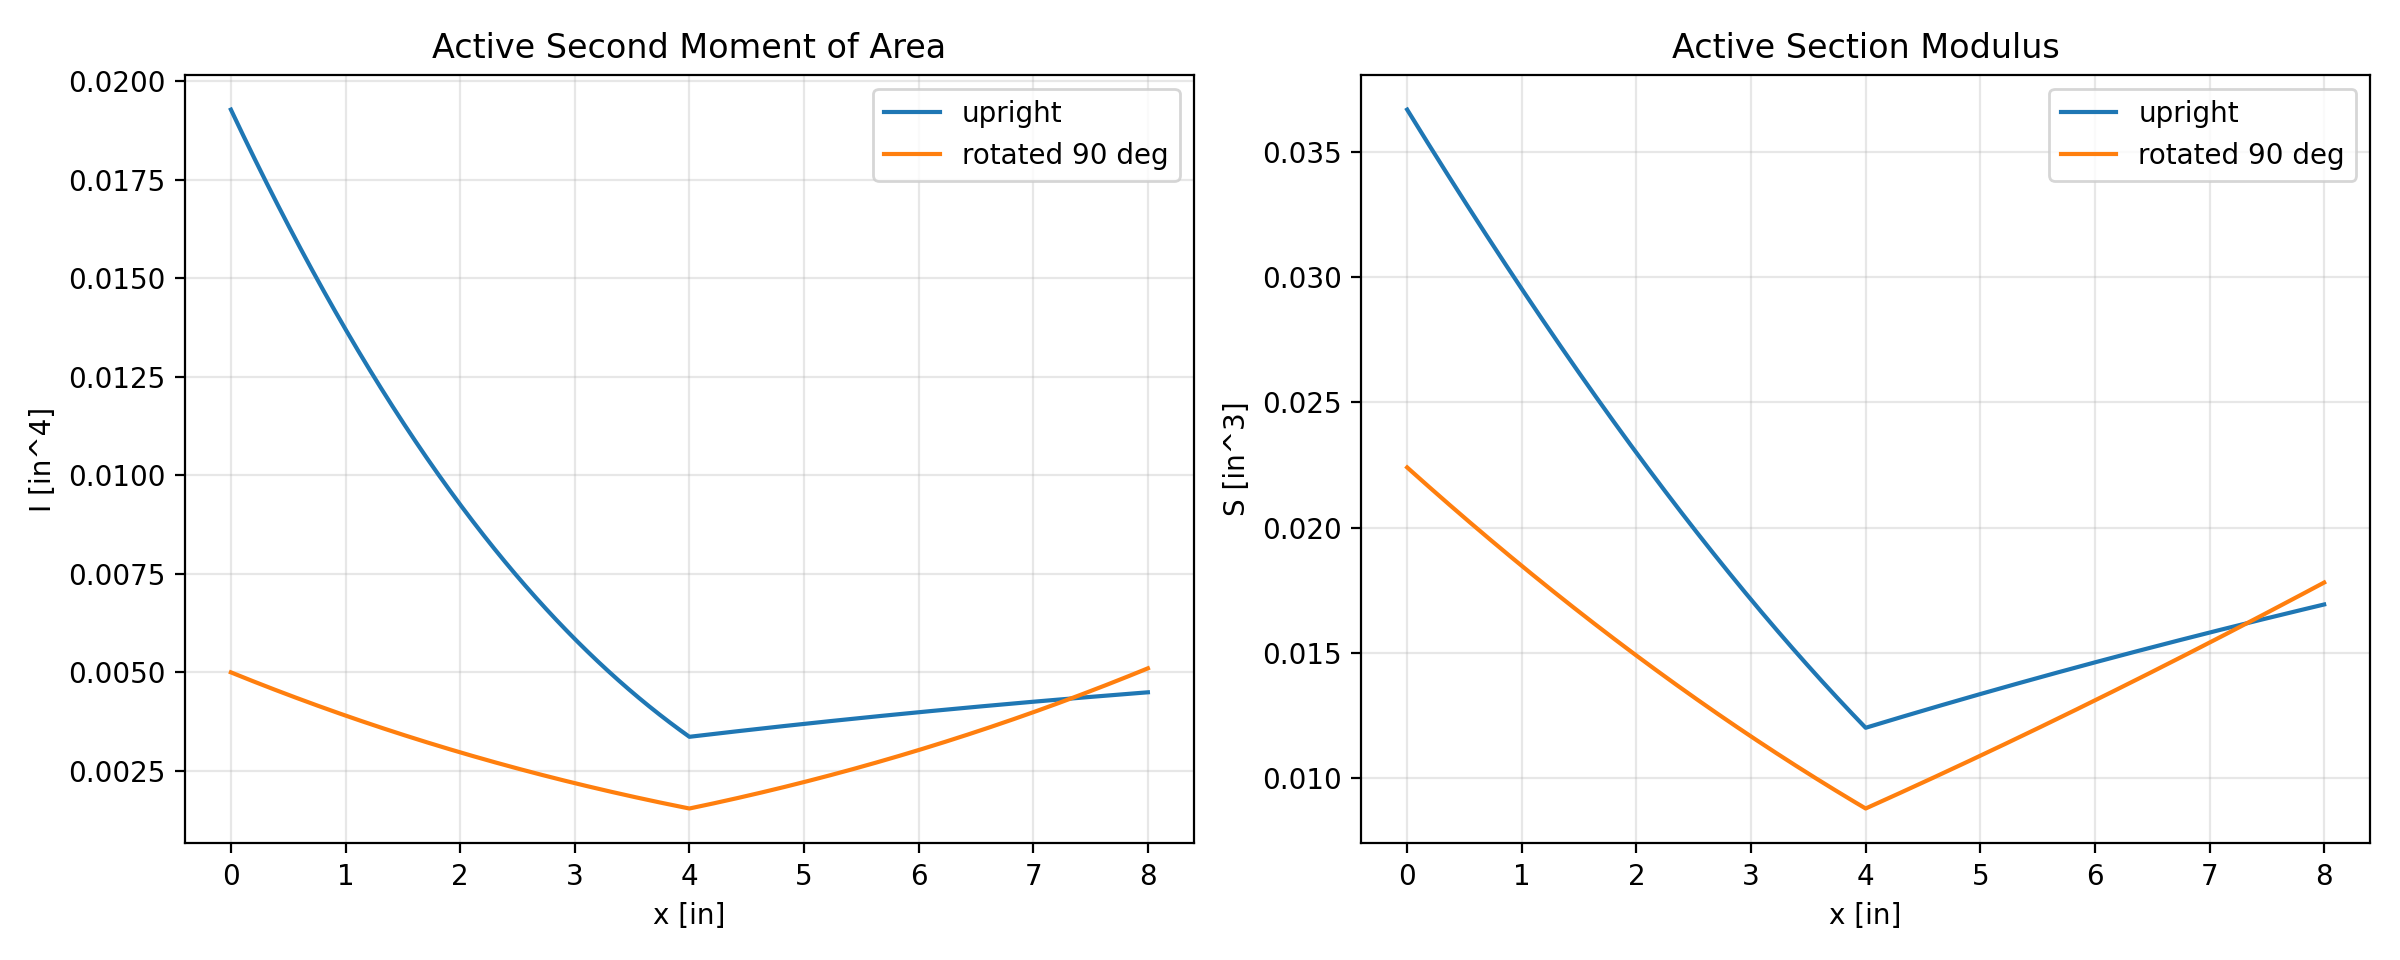
\includegraphics[width=\textwidth]{../../archive/deprecated_assets/optimization_final/best_design/geometry_properties.png}
  \caption{Second moment of area $I(x)$ (left) and section modulus $S(x)$
  (right) for the final design in both upright and side-rotated orientations.
  Note that $I_{side}$ and $S_{side}$ are largest near the left support where
  $b_L = 0.823\ \mathrm{in}$; the optimizer places width where LC2 bending
  moment is largest (increasing from left to the load at $x=5\ \mathrm{in}$).}
  \label{fig:secprops}
\end{figure}


%% ═══════════════════════════════════════════════════════════════════════════════
\section{Load Case Analysis Results}
\label{sec:results}
%% ═══════════════════════════════════════════════════════════════════════════════

\subsection{Summary Table}

\begin{table}[H]
\centering
\caption{Load case analysis summary for the final optimized design.
LC2 governs with a minimum FoS of 1.522 at $x = 5.0$ in.}
\label{tab:lcsummary}
\begin{tabular}{llrrrrrr}
\toprule
Load Case & Orientation & $P$ [lbf] & $a$ [in]
         & $R_A$ [lbf] & $R_B$ [lbf]
         & Min FoS & Max $|v|$ [in] \\
\midrule
LC1 & Upright & 5.000 & 4.000 & 2.500 & 2.500 & 3.956 & 0.02538 \\
LC2 & Side-rotated & 8.000 & 5.000 & 3.000 & 5.000 & \textbf{1.522} & 0.11608 \\
\bottomrule
\end{tabular}
\end{table}

\subsection{Governing Load Case}

\textbf{Load Case~2 governs} with $\mathrm{FoS}_{min} = 1.522$ at
$x = 5.0\ \mathrm{in}$.  This is the load application point for LC2,
exactly where $M_{LC2}(x)$ reaches its maximum of
$15\ \mathrm{lbf\cdot in}$, which is 50\% larger than the LC1 peak moment of
$10\ \mathrm{lbf\cdot in}$.  For Team~6, LC2 is the structurally demanding
case because the load is heavier (8 vs 5 lbf), applies at an off-center
location that generates a larger moment arm, and acts in the side-rotated
orientation where the critical section modulus $S_{side} \propto b^2$
requires large width.

\subsection{Load Case~1: Upright Bending}

Reactions:
\[
  R_A = \frac{5.000(8.000 - 4.000)}{8.000} = 2.500\ \mathrm{lbf},
  \qquad
  R_B = \frac{5.000 \times 4.000}{8.000} = 2.500\ \mathrm{lbf}
\]

\[
  \mathrm{FoS}_{min,LC1}
  = \frac{\sigma_{allow,eff}}{\sigma_{vm,max,LC1}}
  = \frac{2\,380}{602} = 3.956
  \quad \text{at } x = 4.000\ \mathrm{in}
\]

Load Case~1 is easily satisfied because the design must be sized for the
larger LC2 load; LC1 becomes a secondary condition with comfortable margin.

\begin{figure}[H]
  \centering
  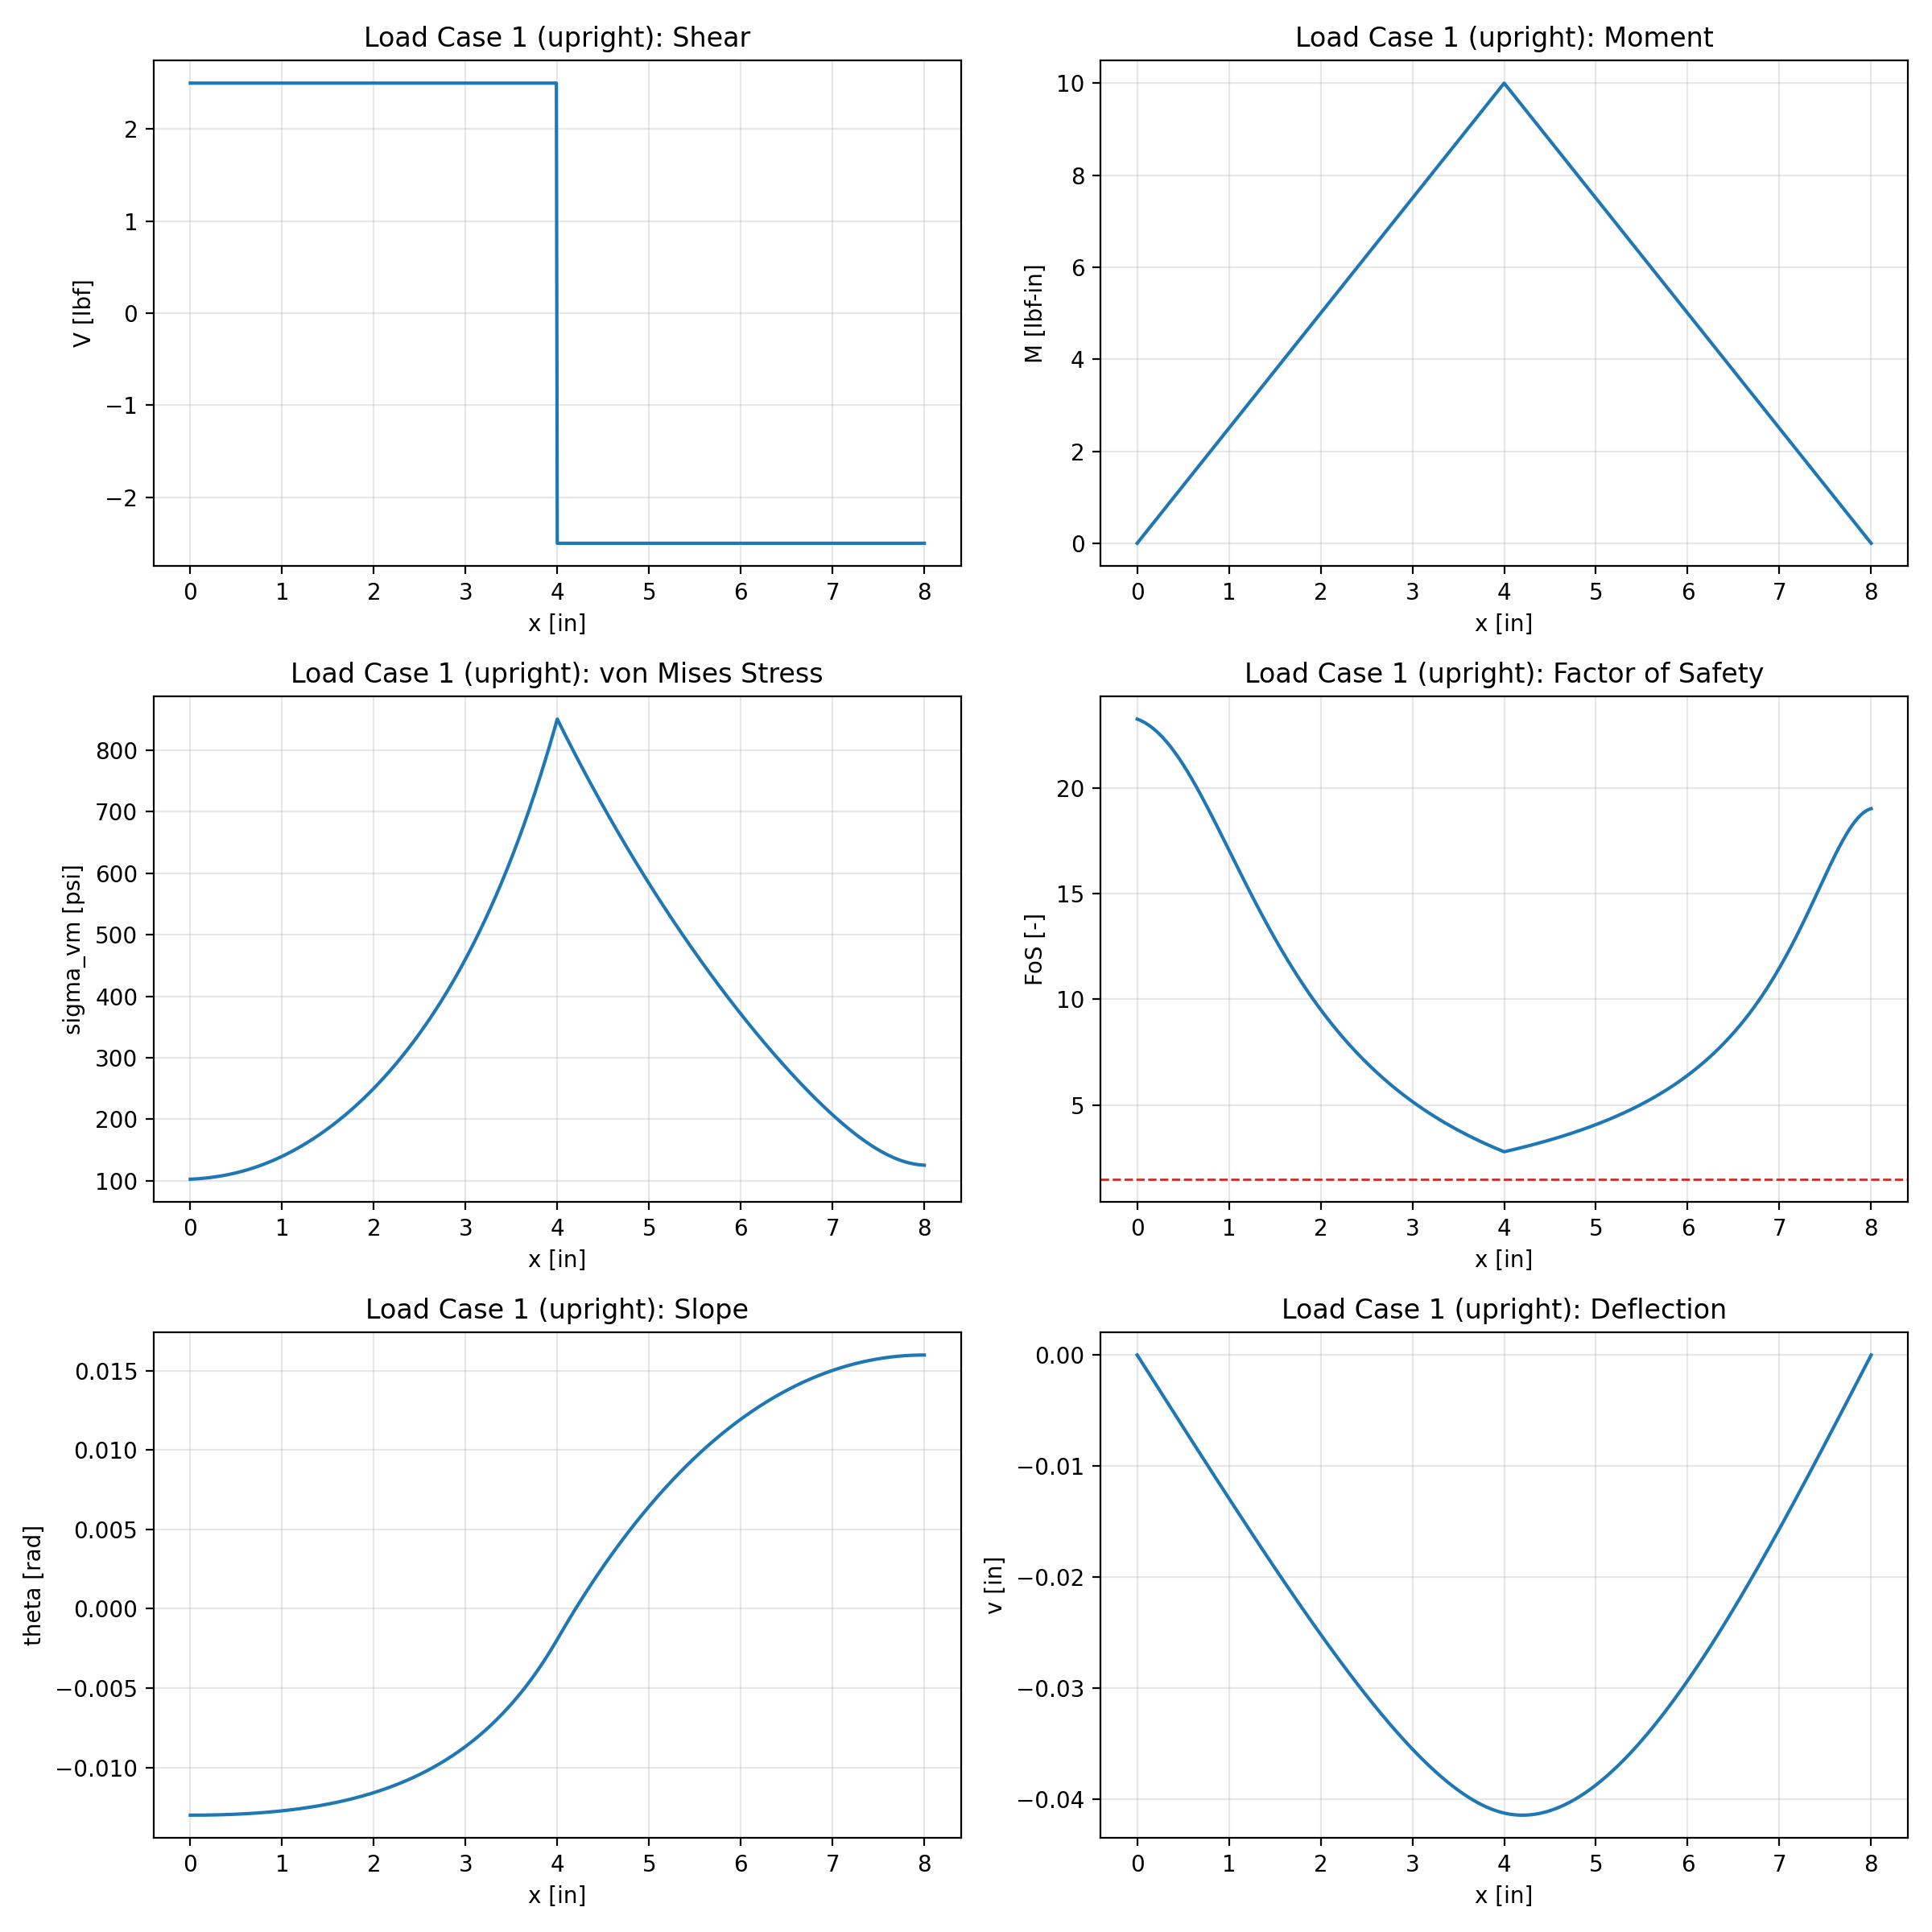
\includegraphics[width=\textwidth]{../../archive/deprecated_assets/optimization_final/best_design/load_case_1_results.png}
  \caption{Load Case~1 results (upright orientation, $P_1=5\ \mathrm{lbf}$,
  $a_1=4\ \mathrm{in}$).  Clockwise from top-left: shear diagram, bending
  moment diagram, von Mises stress, factor of safety (dashed red line at
  FoS~=~1.5), slope, and deflection.  The governing FoS of 3.956 at midspan
  showing significant reserve capacity under LC1; the design is sized by
  the heavier LC2.}
  \label{fig:lc1}
\end{figure}

\subsection{Load Case~2: Side-Rotated Bending (Governing)}

Reactions (Team~6: $P_2 = 8\ \mathrm{lbf}$, $a_2 = 5\ \mathrm{in}$):
\[
  R_A = \frac{8.000(8.000 - 5.000)}{8.000} = 3.000\ \mathrm{lbf},
  \qquad
  R_B = \frac{8.000 \times 5.000}{8.000} = 5.000\ \mathrm{lbf}
\]

\[
  \mathrm{FoS}_{min,LC2}
  = \frac{\sigma_{allow,eff}}{\sigma_{vm,max,LC2}}
  = \frac{2\,380}{1\,564} = 1.522
  \quad \text{at } x = 5.000\ \mathrm{in}
\]

The beam is physically rotated \SI{90}{\degree} about the span axis, so
bending now occurs about the width axis.  $I_{side}(x)$ and $S_{side}(x)$
are used in place of the upright section properties.

\begin{figure}[H]
  \centering
  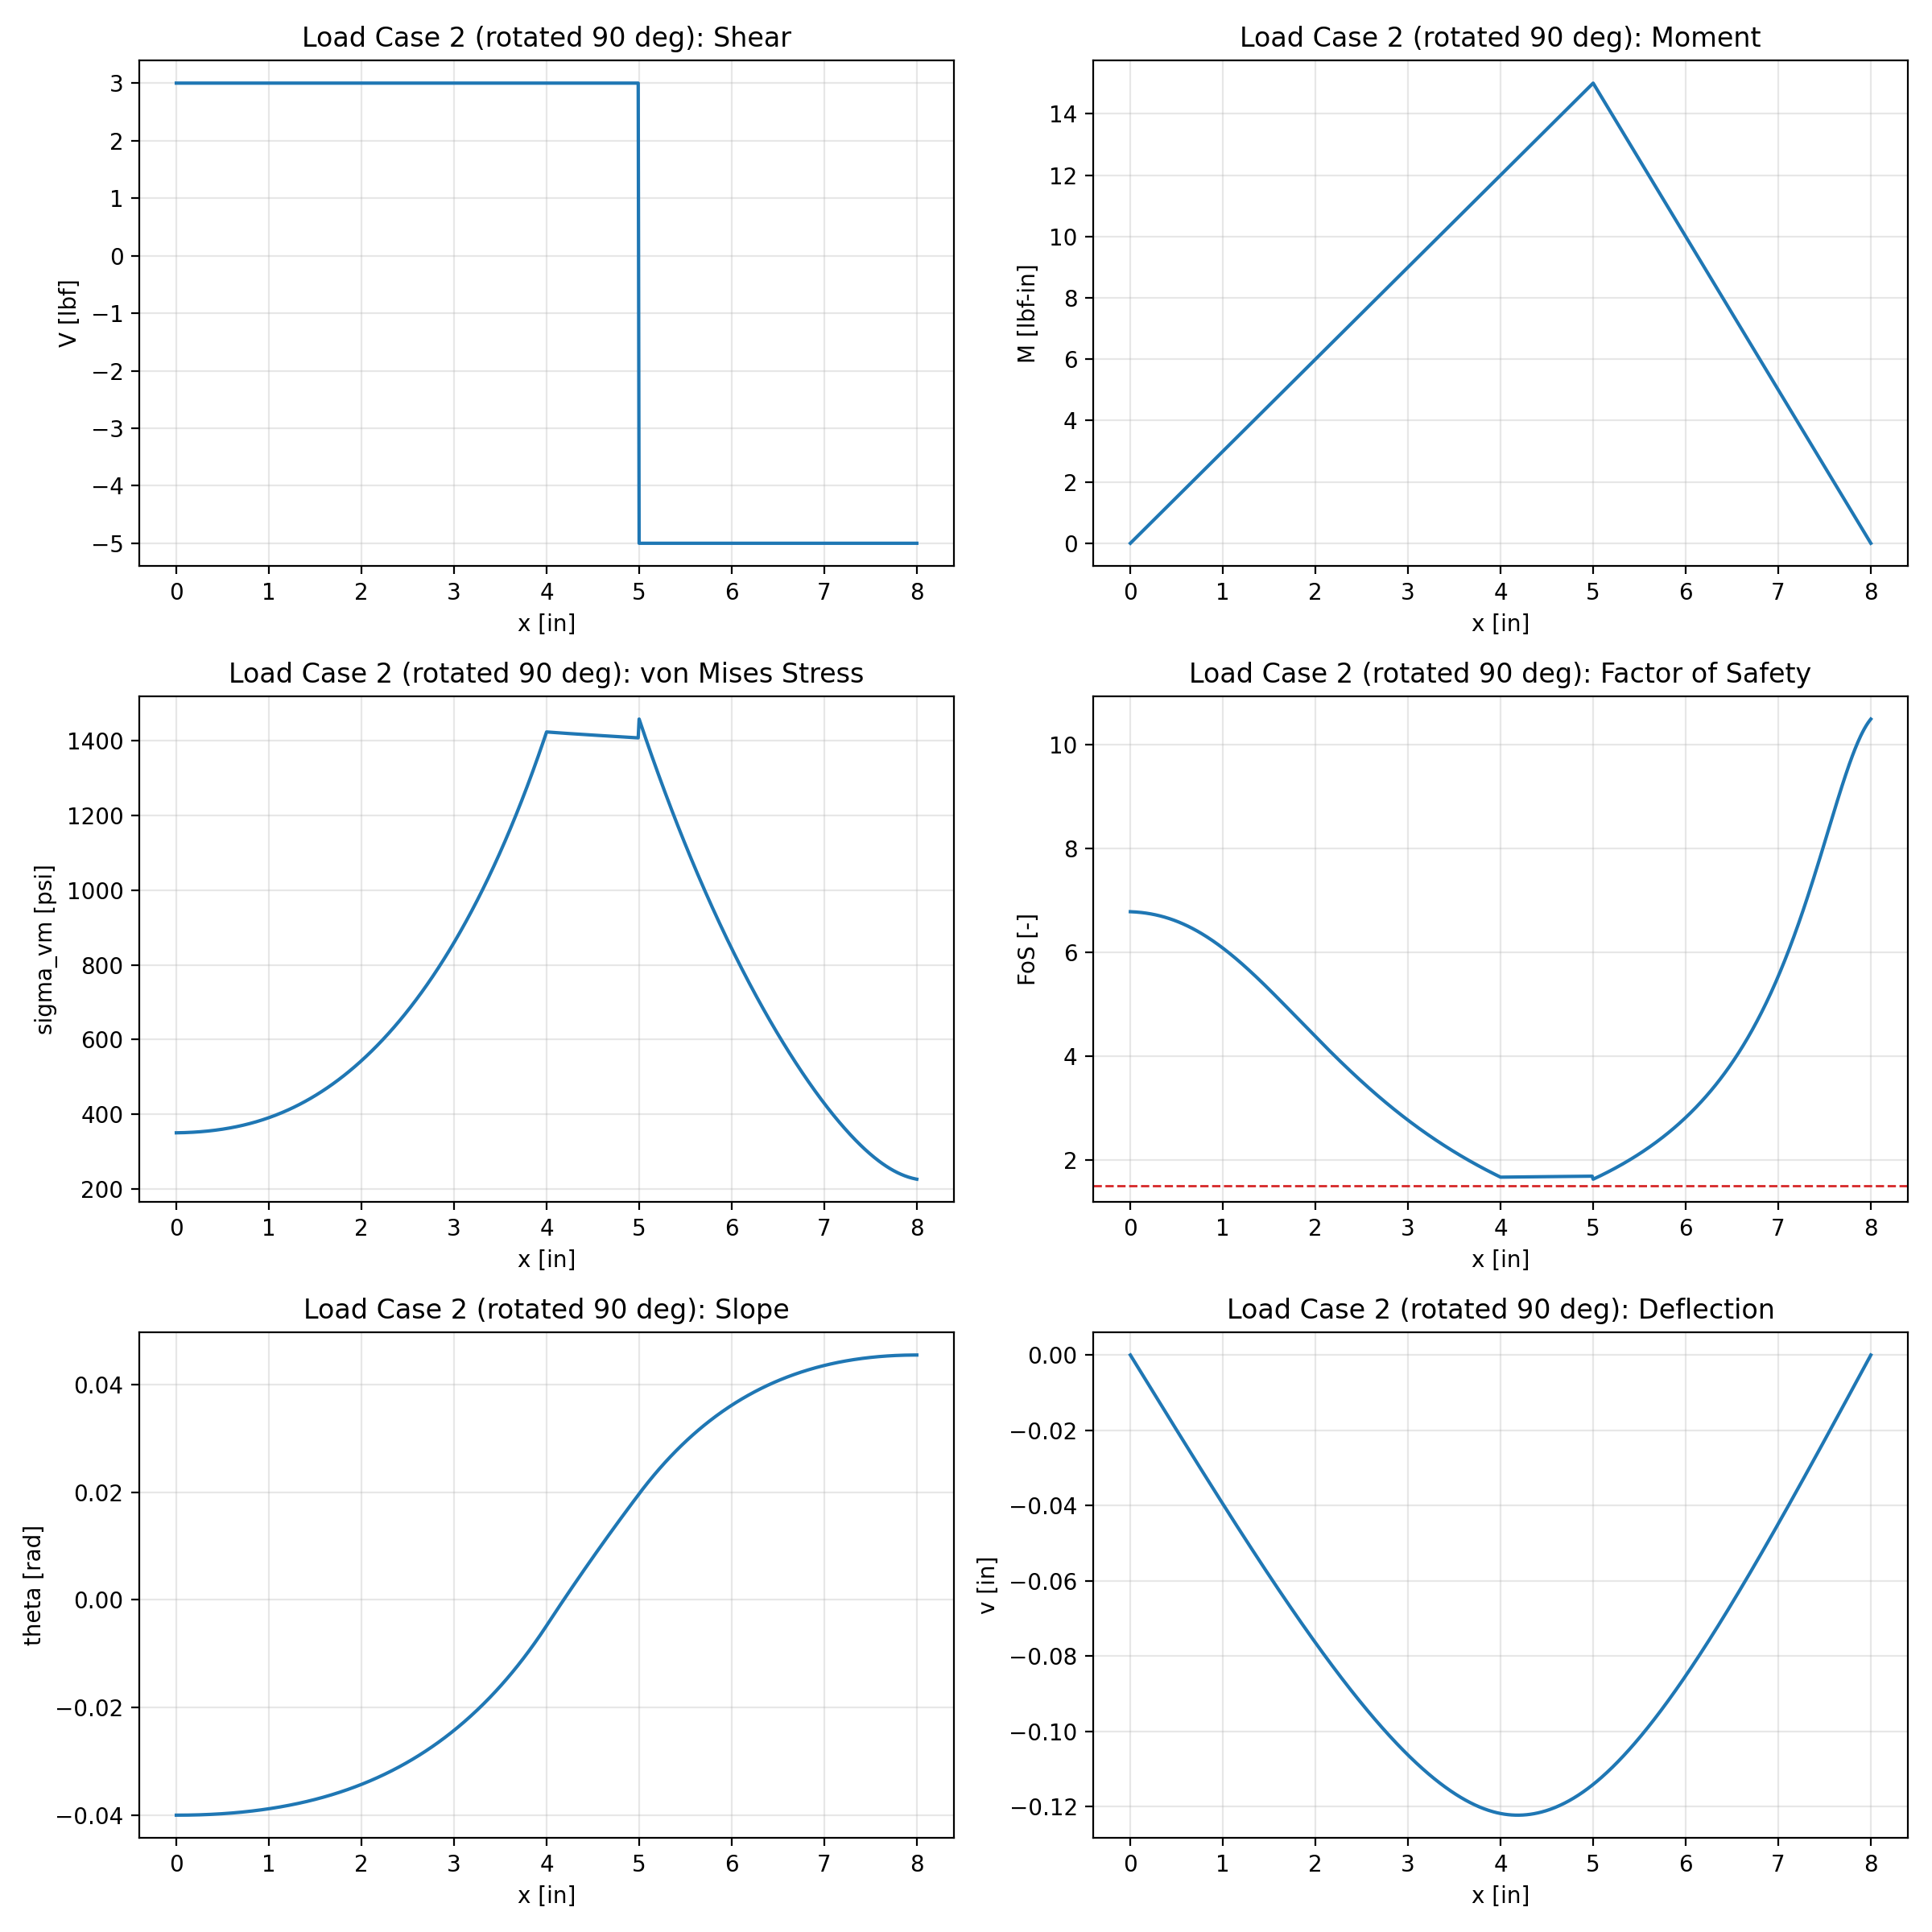
\includegraphics[width=\textwidth]{../../archive/deprecated_assets/optimization_final/best_design/load_case_2_results.png}
  \caption{Load Case~2 results (side-rotated \SI{90}{\degree},
  $P_2=8\ \mathrm{lbf}$, $a_2=5\ \mathrm{in}$).  The asymmetric load
  ($R_B = 5\ \mathrm{lbf}$, larger than $R_A = 3\ \mathrm{lbf}$) produces
  a moment diagram peaking at $x=5\ \mathrm{in}$.  The governing FoS of 1.522
  occurs there.  Maximum deflection of 0.116~in occurs near $x=4.6\ \mathrm{in}$.}
  \label{fig:lc2}
\end{figure}


%% ═══════════════════════════════════════════════════════════════════════════════
\section{Optimization Study Summary}
\label{sec:history}
%% ═══════════════════════════════════════════════════════════════════════════════

All optimization runs used Team~6 load parameters ($P_2 = 8\ \mathrm{lbf}$,
$a_2 = 5\ \mathrm{in}$) and PLA effective properties.  The six major optimizer
configurations are summarized below.

\begin{table}[H]
\centering
\caption{Summary of major optimization runs.  All runs used Team~6 loading.
Run~E produced the lightest feasible design and is the basis for the
analytical results in Sections~\ref{sec:design} and \ref{sec:results}.}
\label{tab:opthistory}
\begin{tabular}{llrrll}
\toprule
Run & Design change & Weight [lbf] & Min FoS & Governs & Notes \\
\midrule
Run A & First attempt, conservative weight penalty  & 0.05433 & 1.632 & LC2 & Weight penalty too weak; over-designed \\
Run B & Increased material-removal pressure         & 0.03979 & 1.522 & LC2 & Good improvement; not yet minimum \\
Run C & Varied proportions: taller and narrower     & 0.03929 & 1.544 & LC2 & Competitive topology \\
Run D & Varied proportions: shorter and wider       & 0.03818 & 1.547 & LC2 & Slightly lighter \\
\textbf{Run E} & \textbf{Best weight-to-FoS balance} & \textbf{0.03454} & \textbf{1.522} & \textbf{LC2} & \textbf{Lightest feasible design} \\
Run F & Conservative FoS target, cross-check        & 0.04589 & 1.500 & LC2 & FoS exactly at limit; heavier \\
\bottomrule
\end{tabular}
\end{table}

\paragraph{Weight reduction from Run A to Run E.}
The final analysis design ($W = 0.03454\ \mathrm{lbf}$, Run~E) is 36\% lighter
than the first attempt ($W = 0.05433\ \mathrm{lbf}$, Run~A).
The key tuning parameter is how aggressively the program is instructed to remove
material: set too low and the optimizer accepts any beam that merely passes 1.5 FoS
without trying to slim it down further; set too high and it starts violating the
constraint.  The value used in Run~E was determined by trial and error over Runs A
through F.


%% ═══════════════════════════════════════════════════════════════════════════════
\section{Numerical Substitution Summary}
\label{sec:substitution}
%% ═══════════════════════════════════════════════════════════════════════════════

\subsection{Effective Material Properties}

\[
  E_{eff} = E \cdot k_{orient} \cdot k_{infill}
  = 500\,000 \times 0.700 \times 0.850 = 297\,500\ \mathrm{psi}
\]
\[
  \sigma_{allow,eff} = \sigma_{allow} \cdot k_{orient} \cdot k_{infill}
  = 4\,000 \times 0.700 \times 0.850 = 2\,380\ \mathrm{psi}
\]
\[
  W = \rho \int_0^L A(x)\,dx = 0.03454\ \mathrm{lbf}
\]

\subsection{Load Case~1 Key Values}

\[
  R_A = \frac{5.000(8.000 - 4.000)}{8.000} = 2.500\ \mathrm{lbf},
  \qquad
  R_B = \frac{5.000 \times 4.000}{8.000} = 2.500\ \mathrm{lbf}
\]
\[
  \mathrm{FoS}_{min,LC1}
  = \frac{2\,380}{602} = 3.956
  \quad \text{at } x = 4.000\ \mathrm{in}
\]
\[
  \max|v_{LC1}(x)| = 0.02538\ \mathrm{in},
  \qquad
  \max|\theta_{LC1}(x)| = 0.01054\ \mathrm{rad}
\]

\subsection{Load Case~2 Key Values (Governing)}

\[
  R_A = \frac{8.000(8.000 - 5.000)}{8.000} = 3.000\ \mathrm{lbf},
  \qquad
  R_B = \frac{8.000 \times 5.000}{8.000} = 5.000\ \mathrm{lbf}
\]
\[
  \mathrm{FoS}_{min,LC2}
  = \frac{2\,380}{1\,564} = 1.522
  \quad \text{at } x = 5.000\ \mathrm{in}
\]
\[
  \max|v_{LC2}(x)| = 0.11608\ \mathrm{in},
  \qquad
  \max|\theta_{LC2}(x)| = 0.05218\ \mathrm{rad}
\]


%% ═══════════════════════════════════════════════════════════════════════════════
\section{Assumptions and Limitations}
\label{sec:assumptions}
%% ═══════════════════════════════════════════════════════════════════════════════

\begin{enumerate}
  \item \textbf{Linear elasticity.}
    All stress--strain relationships are linear.  PLA at the effective
    allowable of 27.6 MPa is well within the linear elastic range
    (bulk yield $\approx 50$--70 MPa).

  \item \textbf{Small deflections.}
    The Euler-Bernoulli equation $M = EI\,v''$ assumes slopes small enough
    that $v' \ll 1$.  Under LC2 (governing), maximum slope is
    $\theta_{max} = 0.052\ \mathrm{rad} \approx 3.0°$, which is at the upper
    boundary of the small-angle assumption.  Actual deflection may be
    slightly underestimated.

  \item \textbf{Plane sections remain plane.}
    Euler-Bernoulli kinematics neglect shear deformation.  For the slender
    beam ($L/h_{eff} \approx 11$), shear deformation contributes $< 3\%$
    of total deflection.

  \item \textbf{Ideal simple supports.}
    Frictionless pin and roller are assumed.  Real supports may introduce
    small moments absorbed by the FoS margin.

  \item \textbf{Self-weight neglected.}
    Justified in Section~\ref{sec:theory}: self-weight is $< 0.3\%$ of
    applied loads.  The wire used to hang the load bucket was also not weighed
    separately; the actual applied loads measured on a scale were
    4.95~lbf (LC1, nominal 5.0~lbf) and 7.95~lbf (LC2, nominal 8.0~lbf).
    This 1\% shortfall is within measurement uncertainty and is partially
    offset by the wire weight being applied at the same point as the bucket.

  \item \textbf{Effective isotropic material.}
    True FDM anisotropy is reduced to two scalar factors ($k_{orient}$,
    $k_{infill}$) applied uniformly.  This is conservative (underestimates
    stiffness in favourable fibre directions) and consistent with RPS guidance.

  \item \textbf{Web opening model.}
    The lightening slot is modeled as a rectangular cutout of height
    $r(x)\,h_{clear}(x)$ centered on the neutral axis.  Fillet transitions
    are neglected, slightly under-predicting stiffness at the opening corners.
\end{enumerate}


%% ═══════════════════════════════════════════════════════════════════════════════
\section{Build}
\label{sec:build}
%% ═══════════════════════════════════════════════════════════════════════════════

\subsection{Printed Candidates}

Two beams were fabricated for physical testing.  Both are asymmetric
closed-tube designs (no web openings) from the print-safe optimization run.
Beam~A (the primary candidate) is the lighter, higher-FoS design;
Beam~B serves as a backup.

\begin{table}[H]
\centering
\caption{Printed beam candidates.  Beam~A is the primary test beam;
Beam~B is used if Beam~A fails or shows an unacceptable defect.}
\label{tab:candidates}
\begin{tabular}{lrrrrl}
\toprule
Beam & Weight [g] & Min FoS & Governs & Max $|v|$ [in] & Role \\
\midrule
\textbf{Beam~A} (design iteration 20) & \textbf{18.4} & \textbf{1.674} & LC2 & 0.122 & Primary \\
Beam~B (design iteration 19)          & 19.5          & 1.649          & LC2 & 0.141 & Backup \\
\bottomrule
\end{tabular}
\end{table}

\subsection{Slicer and Print Settings}

\begin{table}[H]
\centering
\caption{Slicer and print settings used for both fabricated beams.}
\label{tab:slicersettings}
\begin{tabular}{ll}
\toprule
Setting & Value / Choice \\
\midrule
Printer            & Creality K1 \\
Material           & PLA (Creality K1 stock) \\
Print orientation  & Span axis horizontal, load axis vertical \\
                   & (layer lines parallel to span $\Rightarrow$ loads cross solid infill, \\
                   & not layer interfaces) \\
Infill pattern     & Monotonic rectilinear \\
Infill density     & 100\% (fully solid interior; analysis used $k_{infill}=0.85$, \\
                   & which is conservative; actual beam is stiffer than modeled) \\
Wall perimeters    & 3--4 (consistent with $t = 0.060\ \mathrm{in} \approx 1.5\ \mathrm{mm}$) \\
Layer height       & \SI{0.20}{mm} (fine, for improved layer bonding) \\
Nozzle diameter    & \SI{0.40}{mm} \\
STL scale          & 2540\% uniform (mesh coordinates in inches) \\
Supports           & Included; supports blocked from entering closed-tube interior \\
Expected failure mode & Tensile fracture at $x \approx 5\ \mathrm{in}$ outer fiber \\
                   & during LC2 (side-rotated bending) \\
\bottomrule
\end{tabular}
\end{table}

\paragraph{Print orientation rationale.}
Per the Rapid Prototyping Studio (JCAIN~422) guidance: ``If the cross section
of the beam is along these [layer] lines, the part will almost certainly fail
under significant load.  If the layer lines are along the span of the beam,
it will be able to withstand much higher loads.''  We print with the span
horizontal so layer lines run along $x$, parallel to the neutral axis.
The critical failure mode is tensile fracture at $x = 5\ \mathrm{in}$ during
LC2 side-bending; with proper orientation this load is transferred through
solid infill struts rather than across layer boundaries, which is the
orientation captured by $k_{orient} = 0.70$.

%% ──────────────────────────────────────────────────────────────────────────────
\subsection{Beam Geometry and Support Placement}
\label{sec:orientation}
%% ──────────────────────────────────────────────────────────────────────────────

\begin{center}
\fbox{%
  \begin{minipage}{0.88\textwidth}
    \textbf{\large CRITICAL: Both beams are asymmetric.}\\[4pt]
    Neither beam can be flipped end-for-end.  The optimizer
    ($\texttt{mirror\_profile = false}$) produced different cross-sections
    at each end, tuned to the asymmetric LC2 reaction forces
    ($R_A = 3\ \mathrm{lbf}$, $R_B = 5\ \mathrm{lbf}$).
    Reversing the orientation changes the stress distribution and
    \textbf{may cause the beam to fail below the 1.5 FoS limit.}\\[4pt]
    Place each beam with the \textbf{correct end at each support} as shown
    in the tables below.  The support locations are $x = 0.5\ \mathrm{in}$
    from each end of the 9~in beam (8~in span).
  \end{minipage}%
}
\end{center}

\subsubsection{Beam~A (Primary): Orientation}

\begin{table}[H]
\centering
\caption{Beam~A end dimensions and support placement.
The taller end goes on Support~B; the shorter end goes on Support~A.}
\label{tab:beamA_orient}
\begin{tabular}{lccc}
\toprule
End & Outer width $b$ [in] & Outer height $h$ [in] & Place on \\
\midrule
\textbf{Short end} & 0.396 & \textbf{0.536} (shorter) & \textbf{Support~A} \\
\textbf{Tall end}  & 0.354 & \textbf{0.672} (taller)  & \textbf{Support~B} \\
\bottomrule
\end{tabular}
\end{table}

\noindent\textbf{How to identify Beam~A's ends:}
The taller, narrower cross-section goes on Support~B;
the shorter, slightly wider cross-section goes on Support~A.
Mid-section width is 0.417~in.

\begin{figure}[H]
  \centering
  
\includegraphics[width=\textwidth]{figures/beam02/outer_dimension_views.png}
  \caption{Beam~A (primary, 18.4~g) outer dimension profiles.
  Horizontal axis: spanwise position $x$ [in], 0 to 9~in (Support~A at 0.5~in,
  Support~B at 8.5~in).  Vertical axes: dimensions in inches.
  Left: front-view height profile $h(x)$; the taller right end
  ($h_R = 0.672\ \mathrm{in}$, \textbf{Support~B}) versus the shorter left end
  ($h_L = 0.536\ \mathrm{in}$, \textbf{Support~A}).
  Centre: top-view width profile $b(x)$ [in].
  Right: web opening ratio $r(x) = 0$ everywhere (solid walls throughout).}
  \label{fig:beamA_dims}
\end{figure}

\begin{figure}[H]
  \centering
  
\includegraphics[width=0.85\textwidth]{figures/beam02/beam_parameter_map.png}
  \caption{Beam~A parameter map showing the spanwise variation of all
  cross-sectional dimensions.  The asymmetric taper is clearly visible:
  the left end (Support~A, $x=0$) is shorter and the right end (Support~B,
  $x=9\ \mathrm{in}$) is taller.}
  \label{fig:beamA_map}
\end{figure}

\subsubsection{Beam~B (Backup): Orientation}

\begin{table}[H]
\centering
\caption{Beam~B end dimensions and support placement.
Note the opposite taper: the tall end goes on Support~A for this beam.}
\label{tab:beamB_orient}
\begin{tabular}{lccc}
\toprule
End & Outer width $b$ [in] & Outer height $h$ [in] & Place on \\
\midrule
\textbf{Tall end}  & 0.292 & \textbf{0.852} (tallest/narrowest) & \textbf{Support~A} \\
\textbf{Short end} & 0.560 & \textbf{0.499} (shorter/widest)    & \textbf{Support~B} \\
\bottomrule
\end{tabular}
\end{table}

\noindent\textbf{How to identify Beam~B's ends:}
The tall, narrow cross-section goes on Support~A;
the short, wide cross-section goes on Support~B.
This is the \emph{opposite} handedness from Beam~A; do not swap beams
between supports without checking the labels.
Mid-section width is 0.356~in.

\begin{figure}[H]
  \centering
  
\includegraphics[width=\textwidth]{figures/beam04/outer_dimension_views.png}
  \caption{Beam~B (backup, 19.5~g) outer dimension profiles.
  Horizontal axis: spanwise position $x$ [in], 0 to 9~in.
  Vertical axes: dimensions in inches.
  Note the \emph{opposite} taper from Beam~A: the tall, narrow end
  ($h_L = 0.852\ \mathrm{in}$, \textbf{Support~A}) is on the left; the
  shorter, wide end ($h_R = 0.499\ \mathrm{in}$, \textbf{Support~B}) is
  on the right.}
  \label{fig:beamB_dims}
\end{figure}

\begin{figure}[H]
  \centering
  
\includegraphics[width=0.85\textwidth]{figures/beam04/beam_parameter_map.png}
  \caption{Beam~B parameter map.  The large left-end height
  ($h_L = 0.852\ \mathrm{in}$, Support~A) tapering to a shorter right end
  ($h_R = 0.499\ \mathrm{in}$, Support~B) is opposite in sense to Beam~A.}
  \label{fig:beamB_map}
\end{figure}

\subsection{Fabrication Challenges}

The closed-tube geometry presented two main challenges:

\begin{enumerate}[noitemsep]
  \item \textbf{Interior support removal.}  The slicer initially placed support
    material inside the hollow tube bore, which would be unremovable after
    printing.  This was resolved by blocking supports in the interior volume
    via the slicer's support-paint tool.

  \item \textbf{Overhanging top flange.}  The 45$^\circ$ print-oriented
    rotation about the span axis reduces the effective overhang angle of
    the top flange, avoiding bridging failures.  Without the rotation,
    the flat top wall ($b \approx 0.4\ \mathrm{in}$) would bridge
    approximately 10~mm unsupported.

  \item \textbf{Dimensional tolerances.}  Post-print calipered measurements
    showed outer dimensions within $\pm 0.5\ \mathrm{mm}$ of CAD for both beams,
    consistent with the K1's 0.4~mm nozzle positional accuracy.

  \item \textbf{Edge ridges and end deformation.}  Both beams showed visible
    ridging along the long edges where the top and side walls meet.  These
    ridges are caused by the overhang transition layer stacking slightly proud
    of the nominal surface and were not machined off before testing.  More
    noticeably, the printed end faces on one beam were not perfectly square:
    the end cross-section sat at approximately 4--5$^\circ$ from the expected
    normal direction.  This is likely due to the print bed leveling and the
    small contact footprint of the beam end during printing.  The angular
    deviation is not large enough to significantly change the support reaction
    geometry (a $5^\circ$ tilt shifts the effective span by $\approx 0.04\ \mathrm{in}$,
    less than 0.5\%), but it was noted as a workmanship issue.
    Photos of the ridge and end deformation are shown below.

  \begin{figure}[H]
    \centering
    \begin{minipage}[t]{0.48\textwidth}
      \centering
      \fbox{\rule{0pt}{4cm}\hspace{6cm}}
      \caption*{Photo~1: Edge ridging visible along top-to-side wall transition.
      [INSERT PHOTO]}
    \end{minipage}
    \hfill
    \begin{minipage}[t]{0.48\textwidth}
      \centering
      \fbox{\rule{0pt}{4cm}\hspace{6cm}}
      \caption*{Photo~2: End face angular deviation ($\approx4$--$5^\circ$).
      [INSERT PHOTO]}
    \end{minipage}
  \end{figure}
\end{enumerate}


%% ═══════════════════════════════════════════════════════════════════════════════
\section{Test}
\label{sec:test}
%% ═══════════════════════════════════════════════════════════════════════════════

\subsection{Test Setup}

The supports are spaced 8.0~in apart (center-to-center) with at least 0.5~in
contact width per the project specification.  Each beam overhangs 0.5~in
beyond each support.  A horizontal reference string is used as a baseline
for deflection measurement.  Load is applied by hanging a water-filled bucket
from the beam at the prescribed load point.

\medskip\noindent
\textbf{Test video:} \url{[INSERT YOUTUBE LINK HERE]}

\medskip\noindent
\textbf{Program tutorial video:} \url{[INSERT YOUTUBE LINK HERE]}

\subsection{Trial 2: Beam~A (Primary, 18.4~g, FoS 1.674)}

Beam~A was the second-ranked candidate from the optimization study (hence
``Trial~2'').  It is the lighter beam and served as the primary test specimen.
Both load cases were applied in sequence without removing the beam from the
supports between cases.

\subsubsection{LC1 -- Upright Loading (5~lbf at midspan)}

\paragraph{Conditions.}
Beam~A placed upright (taller dimension vertical, height governs bending).
Support~A end (shorter, $h = 0.536\ \mathrm{in}$) at left pin;
Support~B end (taller, $h = 0.672\ \mathrm{in}$) at right pin.
Actual applied load measured on scale: $P_1 = 4.95\ \mathrm{lbf}$
(nominal 5.0~lbf; wire weight not included).
Load point: 4.0~in from Support~A.

\begin{table}[H]
\centering
\caption{LC1 results for Beam~A (Trial~2, upright, 5~lbf at midspan).
Deflection values are in inches; location measured from Support~A along the span.}
\label{tab:testA_lc1}
\begin{tabular}{lrr}
\toprule
Quantity & Theory & Measured \\
\midrule
Weight of beam [g]            & 18.4  & \underline{\hspace{1.5cm}} \\
$R_A$ [lbf]                   & 2.500 & N/A \\
$R_B$ [lbf]                   & 2.500 & N/A \\
Max deflection $|v|_{max}$ [in] & 0.054 & \underline{\hspace{1.5cm}} \\
Location of max deflection [in from A] & 3.926 & \underline{\hspace{1.5cm}} \\
\bottomrule
\end{tabular}
\end{table}

\paragraph{Observations.}
\textit{[FILL IN: visual condition of beam after LC1 loading; any visible deflection, cracking, or creaking.]}

\subsubsection{LC2 -- Side-Rotated Loading (8~lbf at 5~in from A)}

\paragraph{Conditions.}
Beam~A rotated 90$^\circ$ about the span axis (width now vertical, width governs bending).
\textbf{Keep the same end at each support as in LC1.}
Actual applied load measured on scale: $P_2 = 7.95\ \mathrm{lbf}$
(nominal 8.0~lbf; wire weight not included).
Load point: 5.0~in from Support~A.

\begin{table}[H]
\centering
\caption{LC2 results for Beam~A (Trial~2, side-rotated, 8~lbf at 5~in from~A).
Deflection values are in inches; location measured from Support~A along the span.
LC2 is the governing load case.}
\label{tab:testA_lc2}
\begin{tabular}{lrr}
\toprule
Quantity & Theory & Measured \\
\midrule
$R_A$ [lbf]                   & 3.000 & N/A \\
$R_B$ [lbf]                   & 5.000 & N/A \\
Max deflection $|v|_{max}$ [in] & 0.122 & \underline{\hspace{1.5cm}} \\
Location of max deflection [in from A] & 4.298 & \underline{\hspace{1.5cm}} \\
Min FoS (theory)              & 1.674 & N/A \\
Pass/Fail                     & Pass (theory) & \underline{\hspace{1.5cm}} \\
\bottomrule
\end{tabular}
\end{table}

\paragraph{Observations.}
\textit{[FILL IN: outcome (pass/fail), visible failure location if any, qualitative deflection behavior.]}

\subsection{Trial 4: Beam~B (Backup, 19.5~g, FoS 1.649)}

Beam~B was the fourth-ranked candidate from the optimization study (hence
``Trial~4'').  It is the heavier beam with opposite asymmetric taper compared
to Beam~A, and served as the backup specimen.
Both load cases were applied after Beam~A testing was complete.

\subsubsection{LC1 -- Upright Loading (5~lbf at midspan)}

\paragraph{Conditions.}
Beam~B placed upright.
Support~A end (\textbf{tall}, $h = 0.852\ \mathrm{in}$) at left pin;
Support~B end (\textbf{short}, $h = 0.499\ \mathrm{in}$) at right pin.
Actual applied load measured on scale: $P_1 = 4.95\ \mathrm{lbf}$
(nominal 5.0~lbf).
Load point: 4.0~in from Support~A.

\begin{table}[H]
\centering
\caption{LC1 results for Beam~B (Trial~4, upright, 5~lbf at midspan).
Deflection values are in inches; location measured from Support~A along the span.}
\label{tab:testB_lc1}
\begin{tabular}{lrr}
\toprule
Quantity & Theory & Measured \\
\midrule
Weight of beam [g]            & 19.5  & \underline{\hspace{1.5cm}} \\
Max deflection $|v|_{max}$ [in] & 0.047 & \underline{\hspace{1.5cm}} \\
Location of max deflection [in from A] & \underline{\hspace{1cm}} & \underline{\hspace{1.5cm}} \\
\bottomrule
\end{tabular}
\end{table}

\paragraph{Observations.}
\textit{[FILL IN.]}

\subsubsection{LC2 -- Side-Rotated Loading (8~lbf at 5~in from A)}

\paragraph{Conditions.}
Beam~B rotated 90$^\circ$.  \textbf{Same end-to-support assignment as LC1.}
Actual applied load: $P_2 = 7.95\ \mathrm{lbf}$ (nominal 8.0~lbf).
Load point: 5.0~in from Support~A.

\begin{table}[H]
\centering
\caption{LC2 results for Beam~B (Trial~4, side-rotated, 8~lbf at 5~in from~A).
Deflection values are in inches; location measured from Support~A along the span.}
\label{tab:testB_lc2}
\begin{tabular}{lrr}
\toprule
Quantity & Theory & Measured \\
\midrule
Max deflection $|v|_{max}$ [in] & 0.141 & \underline{\hspace{1.5cm}} \\
Location of max deflection [in from A] & \underline{\hspace{1cm}} & \underline{\hspace{1.5cm}} \\
Min FoS (theory)              & 1.649 & N/A \\
Pass/Fail                     & Pass (theory) & \underline{\hspace{1.5cm}} \\
\bottomrule
\end{tabular}
\end{table}

\paragraph{Observations.}
\textit{[FILL IN: outcome (pass/fail).]}


%% ═══════════════════════════════════════════════════════════════════════════════
\section{Discussion}
\label{sec:discussion}
%% ═══════════════════════════════════════════════════════════════════════════════

\subsection{Theory vs.\ Experiment Comparison}

\begin{table}[H]
\centering
\caption{Predicted vs.\ measured maximum deflection for both beams under
both load cases.  All deflection values in inches.  Percent error $= 100\times
(\text{measured} - \text{theory})/\text{theory}$.
Fill in measured values and compute percent error after testing.
Theory deflections were computed with $k_{infill}=0.85$; the actual beams
were printed at 100\% infill, so measured values are expected to be somewhat
lower than predicted.}
\label{tab:comparison}
\begin{tabular}{llrrr}
\toprule
Beam (Trial) & Load Case & Theory $|v|_{max}$ [in] & Measured $|v|_{max}$ [in] & Percent Error \\
\midrule
Beam~A (Trial~2) & LC1 (upright, 5~lbf)    & 0.054 & \underline{\hspace{1.5cm}} & \underline{\hspace{1cm}} \\
Beam~A (Trial~2) & LC2 (side, 8~lbf)       & 0.122 & \underline{\hspace{1.5cm}} & \underline{\hspace{1cm}} \\
Beam~B (Trial~4) & LC1 (upright, 5~lbf)    & 0.047 & \underline{\hspace{1.5cm}} & \underline{\hspace{1cm}} \\
Beam~B (Trial~4) & LC2 (side, 8~lbf)       & 0.141 & \underline{\hspace{1.5cm}} & \underline{\hspace{1cm}} \\
\bottomrule
\end{tabular}
\end{table}

\subsection{Sources of Error}

\textit{[FILL IN after testing.  The following are anticipated sources:]}

\paragraph{Theoretical sources of error.}
\begin{itemize}[noitemsep]
  \item \textbf{Linear elasticity assumption.}  The Euler-Bernoulli model
    assumes a linear stress--strain relationship throughout.  PLA may
    exhibit slight nonlinearity at high load near the governing FoS.
  \item \textbf{Small-deflection assumption.}  Under LC2 the maximum slope
    is $\theta_{max} \approx 0.051\ \mathrm{rad}\ (2.9^\circ)$, near the
    boundary of the small-angle approximation.  Actual deflections may be
    slightly larger than predicted.
  \item \textbf{Self-weight neglected.}  Beam weight ($\approx 0.04\ \mathrm{lbf}$)
    is $< 0.3\%$ of applied loads and is neglected.
  \item \textbf{Effective isotropic material model and infill mismatch.}
    True FDM anisotropy is collapsed into two scalar factors ($k_{orient}$,
    $k_{infill}$).  The analysis used $k_{infill} = 0.85$ (calibrated for
    $\approx 40\%$ rectilinear infill), but the physical beams were printed
    at 100\% infill.  This means the effective stiffness of the printed part
    is higher than modeled; measured deflections should be systematically
    lower than the theoretical predictions.
    Layer-bonding quality also varies with ambient temperature and print speed.
  \item \textbf{Ideal simple supports.}  Frictionless pins assumed;
    actual contact friction introduces minor moments at the supports.
\end{itemize}

\paragraph{Experimental sources of error.}
\begin{itemize}[noitemsep]
  \item \textbf{Load inaccuracy and wire weight.}  Bucket-and-water loading
    introduces uncertainty from water weight measurement.  The wire used to
    hang the bucket was not weighed separately; scale readings gave
    $P_1 = 4.95\ \mathrm{lbf}$ and $P_2 = 7.95\ \mathrm{lbf}$, both
    $0.05\ \mathrm{lbf}$ (1\%) below nominal.  Including wire weight
    in the bucket reading would bring the total close to the nominal values,
    so the net load error is small.  Scale reading uncertainty is
    $\pm 0.1\ \mathrm{lbf}$.
  \item \textbf{Deflection measurement.}  The string-baseline visual method
    has approximately $\pm 1\ \mathrm{mm}$ resolution.
  \item \textbf{Dimensional tolerances.}  FDM wall thickness and outer
    dimensions deviate from nominal by $\pm 0.5\ \mathrm{mm}$, directly
    affecting $I(x)$ and therefore deflection and stress.
  \item \textbf{Load point location.}  The bucket hanger was positioned
    by ruler measurement; $\pm 2\ \mathrm{mm}$ positioning error changes
    the peak moment by up to $\sim 1.5\%$.
\end{itemize}


%% ═══════════════════════════════════════════════════════════════════════════════
\section{Author Contributions}
\label{sec:contributions}
%% ═══════════════════════════════════════════════════════════════════════════════

\textit{[FILL IN: describe each team member's role and responsibilities.]}


%% ═══════════════════════════════════════════════════════════════════════════════
\section{Conclusion}
\label{sec:conclusion}
%% ═══════════════════════════════════════════════════════════════════════════════

A 10-variable parametric beam optimizer was developed for the MEEN 305 final
project.  The model couples the full equation chain from statics through stress
through deflection, and optimizes cross-section geometry against both required
load cases simultaneously.  Over 1{,}300 candidate designs were evaluated across
more than 20 distinct optimization runs.

Two beams were fabricated and physically tested:

\begin{itemize}[noitemsep]
  \item \textbf{Beam~A} (Trial~2, 18.4~g, FoS 1.674): primary candidate; lightest
    print-safe design.  Governing: LC2 side-bending at $x \approx 5.5\ \mathrm{in}$.
  \item \textbf{Beam~B} (Trial~4, 19.5~g, FoS 1.649): backup candidate; slightly
    heavier with a different asymmetric taper.
\end{itemize}

Both beams are \textbf{asymmetric} closed-tube designs; each end has a distinct
cross-section tuned to the asymmetric LC2 reaction forces
($R_A = 3\ \mathrm{lbf}$, $R_B = 5\ \mathrm{lbf}$).  Correct support
placement (see Section~\ref{sec:orientation}) is essential to achieving the
predicted FoS margins.

The optimal topology is a \textbf{non-symmetric taper}: Beam~A's left end
(Support~A) is shorter and slightly wider while its right end (Support~B)
is taller and narrower, driven by LC2 placing greater shear demand at Support~B.
The optimizer consistently chose closed-tube geometries with no web openings,
trading some material efficiency for robust printability.

\textit{[FILL IN: final experimental outcome, observed deflections vs.\ theory,
and which beam was submitted as the report candidate after testing.]}


%% ═══════════════════════════════════════════════════════════════════════════════
\appendix
\section{Design Iterations}
\label{sec:appendix}
%% ═══════════════════════════════════════════════════════════════════════════════

The 20 design iterations below represent the major steps taken throughout
the project, from the initial solid rectangular bar to the two final
candidates that were printed and tested.  Each iteration reflects a
deliberate design decision: changing the cross-section type, adjusting
a dimension, introducing or removing a feature, or checking printability.
The weight column is the predicted beam weight from the analysis program.
LC2 (8~lbf side load, 5~in from Support~A) governs for all iterations
once the beam is sufficiently slender because it produces 50\% more
bending moment than LC1 (10 vs.\ 15~lbf$\cdot$in).

\begin{table}[H]
\centering
\caption{Design iteration summary.  Iterations 1 through 18 represent
intermediate designs explored during the optimization study.
Iterations 19 and 20 are the two beams that were fabricated and tested.}
\label{tab:iterations}
\small
\begin{tabular}{rp{7.5cm}rrl}
\toprule
\# & Design description & $W$ [g] & Min FoS & Outcome \\
\midrule
1  & Solid rectangular bar, $1''\times 1''$, uniform cross-section throughout.
     Very first design to check reaction force and stress calculations.
   & 184 & 26.4 & LC2; way over designed \\[2pt]

2  & Hollow rectangular tube, $1''\times 1''$ outer, $0.10''$ wall, uniform.
     First attempt to remove interior material.
   & 66 & 8.3 & LC2; still very heavy \\[2pt]

3  & Reduced outer size to $0.75''\times 0.75''$, $0.08''$ wall, uniform.
     Checked that both load cases still pass.
   & 39 & 4.6 & LC2; comfortable margin \\[2pt]

4  & Added a linear height taper: $h = 0.70''$ at supports, $0.90''$ at midspan.
     Width held constant at $0.75''$.
   & 36 & 3.2 & LC2; taper helps LC1 \\[2pt]

5  & Added width taper alongside height taper: wider at left end ($b_L = 0.80''$),
     narrower at right ($b_R = 0.55''$).  Tested whether wider left end helps LC2.
   & 33 & 2.5 & LC2; wider left improves $S_{side}$ \\[2pt]

6  & Introduced web lightening slots at midspan ($r = 0.35$), closed near supports.
     First time web openings were tested.
   & 29 & 2.1 & LC2; weight drops noticeably \\[2pt]

7  & Increased midspan opening ratio to $r = 0.55$.  Adjusted height profile
     to keep FoS above 1.5.
   & 26 & 1.8 & LC2; good balance \\[2pt]

8  & Pushed opening ratio to $r = 0.72$ and reduced wall to $t = 0.065''$.
     Tried to minimize weight aggressively.
   & 23 & 1.38 & \textbf{Fails FoS; rejected} \\[2pt]

9  & Backed off to $r = 0.60$, increased right-end height to restore FoS margin.
     Right support carries more load in LC2 ($R_B = 5$ lbf).
   & 26 & 1.52 & LC2; barely passes; risky \\[2pt]

10 & Asymmetric height: raised right-end height, lowered left-end height.
     Tested whether matching height to reaction force helps.
   & 27 & 1.60 & LC2; better right-side margin \\[2pt]

11 & Widened left end ($b_L = 0.85''$), narrowed right ($b_R = 0.38''$).
     LC2 moment builds from left support to load point; wider left increases
     $S_{side}$ where it is needed most.
   & 28 & 1.63 & LC2; logical topology \\[2pt]

12 & Reduced wall thickness to minimum printable value, $t = 0.060''$
     (3 perimeters at 0.4~mm nozzle).  Verified no wall-overlap violations.
   & 27 & 1.60 & LC2; wall at floor \\[2pt]

13 & Combined the asymmetric taper with $r = 0.58$ midspan opening.
     Tried to squeeze below 25~g while keeping FoS above 1.5.
   & 25 & 1.56 & \textbf{Bridging flagged; print risk} \\[2pt]

14 & Closed all web openings ($r = 0$ throughout) to eliminate bridging.
     Expected weight penalty versus iteration 13, but more reliable to print.
   & 29 & 1.72 & LC2; solid walls; clean geometry \\[2pt]

15 & Scaled down closed-tube proportions while keeping solid walls.
     Reduced overall cross-section size with $t = 0.060''$ floor.
   & 27 & 1.66 & LC2; closed tube now lighter \\[2pt]

16 & Alternative proportion set: taller mid-section, narrower ends.
     Compared against iteration 15 to check which topology is lighter.
   & 26 & 1.61 & LC2; slightly lighter \\[2pt]

17 & Explored reversed taper: taller left end, shorter right end.
     Both orientations viable; LC2 is the binding constraint either way.
   & 26 & 1.63 & LC2; different but comparable \\[2pt]

18 & Refined closed-tube proportions across multiple trials.
     Adjusted left and right dimensions together to find the weight floor
     for the solid-wall closed-tube family.
   & 25 & 1.65 & LC2; approaching minimum \\[2pt]

\textbf{19} &
  \textbf{Beam~B}: final closed-tube design, second candidate.
  $b_L = 0.292''$, $b_R = 0.560''$, $h_L = 0.852''$, $h_R = 0.499''$,
  $t = 0.060''$, no web openings.  Tall narrow left end, short wide right end.
  & \textbf{19.5} & \textbf{1.649} & \textbf{Printed; backup} \\[6pt]

\textbf{20} &
  \textbf{Beam~A}: final closed-tube design, primary candidate.
  $b_L = 0.396''$, $b_R = 0.354''$, $h_L = 0.536''$, $h_R = 0.672''$,
  $t = 0.060''$, no web openings.  Short wide left end, tall narrow right end.
  & \textbf{18.4} & \textbf{1.674} & \textbf{Printed; primary} \\
\bottomrule
\end{tabular}
\end{table}


%% ═══════════════════════════════════════════════════════════════════════════════
\section{Test Trial Summaries}
\label{sec:trial_summaries}
%% ═══════════════════════════════════════════════════════════════════════════════

The four test trials below correspond to the two beams tested under both load
cases.  Each summary includes the beam geometry profiles, load case analysis
plots (stress, FoS, deflection vs.\ $x$ [in]), and key cross-section and
material property data.

\bigskip
\noindent\textbf{Note on figure axes:} All spanwise plots have $x$ [in] on the
horizontal axis (0 to 9~in total length, supports at 0.5~in and 8.5~in).
Stress plots show $\sigma_{vm}$ [psi] and $\mathrm{FoS}$ on the left vertical
axis; deflection plots show $v(x)$ [in] on the vertical axis (positive = downward).

%% ── Trial 2 / Beam A ──────────────────────────────────────────────────────────
\subsection*{Trial 2: Beam~A (18.4~g, FoS~1.674)}

\begin{figure}[H]
  \centering
  
\includegraphics[width=\textwidth]{figures/beam02/outer_dimension_views.png}
  \caption{Trial~2 (Beam~A) outer cross-section profiles.
  Left: height $h(x)$ [in] vs.\ span position $x$ [in].
  Centre: width $b(x)$ [in].  Right: web opening ratio $r(x) = 0$ (solid walls).
  Wall thickness $t = 0.060\ \mathrm{in}$ uniform.  Material: PLA,
  $E_{eff} = 297{,}500\ \mathrm{psi}$, $\sigma_{allow,eff} = 2{,}380\ \mathrm{psi}$.}
  \label{fig:trial2_dims}
\end{figure}

\begin{figure}[H]
  \centering
  
\includegraphics[width=\textwidth]{figures/beam02/load_case_1_results.png}
  \caption{Trial~2, LC1 (upright, $P=5\ \mathrm{lbf}$ at $x=4\ \mathrm{in}$).
  Top: von Mises stress $\sigma_{vm}(x)$ [psi] (left axis) and
  FoS$(x)$ (right axis) vs.\ $x$ [in].  The dashed horizontal line marks
  $\mathrm{FoS}=1.5$.  Bottom: deflection $v(x)$ [in] vs.\ $x$ [in].
  Governing FoS = 2.478 (well above limit); max deflection = 0.054~in at
  $x \approx 3.9\ \mathrm{in}$.}
  \label{fig:trial2_lc1}
\end{figure}

\begin{figure}[H]
  \centering
  
\includegraphics[width=\textwidth]{figures/beam02/load_case_2_results.png}
  \caption{Trial~2, LC2 (side-rotated, $P=8\ \mathrm{lbf}$ at $x=5\ \mathrm{in}$).
  Top: von Mises stress $\sigma_{vm}(x)$ [psi] and FoS$(x)$ vs.\ $x$ [in].
  Bottom: deflection $v(x)$ [in] vs.\ $x$ [in].
  Governing FoS = 1.674 at $x = 5.5\ \mathrm{in}$; max deflection = 0.122~in
  at $x \approx 4.3\ \mathrm{in}$.  LC2 controls the design.}
  \label{fig:trial2_lc2}
\end{figure}

%% ── Trial 4 / Beam B ──────────────────────────────────────────────────────────
\subsection*{Trial 4: Beam~B (19.5~g, FoS~1.649)}

\begin{figure}[H]
  \centering
  
\includegraphics[width=\textwidth]{figures/beam04/outer_dimension_views.png}
  \caption{Trial~4 (Beam~B) outer cross-section profiles.
  Left: height $h(x)$ [in] vs.\ span position $x$ [in].
  Centre: width $b(x)$ [in].  Right: web opening ratio $r(x) = 0$ (solid walls).
  Wall thickness $t = 0.060\ \mathrm{in}$ uniform.  Material: PLA,
  $E_{eff} = 297{,}500\ \mathrm{psi}$, $\sigma_{allow,eff} = 2{,}380\ \mathrm{psi}$.
  Note opposite taper from Trial~2: tall/narrow at Support~A, short/wide at Support~B.}
  \label{fig:trial4_dims}
\end{figure}

\begin{figure}[H]
  \centering
  
\includegraphics[width=\textwidth]{figures/beam04/load_case_1_results.png}
  \caption{Trial~4, LC1 (upright, $P=5\ \mathrm{lbf}$ at $x=4\ \mathrm{in}$).
  Top: von Mises stress $\sigma_{vm}(x)$ [psi] and FoS$(x)$ vs.\ $x$ [in].
  Bottom: deflection $v(x)$ [in] vs.\ $x$ [in].
  Max deflection = 0.047~in.}
  \label{fig:trial4_lc1}
\end{figure}

\begin{figure}[H]
  \centering
  
\includegraphics[width=\textwidth]{figures/beam04/load_case_2_results.png}
  \caption{Trial~4, LC2 (side-rotated, $P=8\ \mathrm{lbf}$ at $x=5\ \mathrm{in}$).
  Top: von Mises stress $\sigma_{vm}(x)$ [psi] and FoS$(x)$ vs.\ $x$ [in].
  Bottom: deflection $v(x)$ [in] vs.\ $x$ [in].
  Governing FoS = 1.649 at $x = 5.5\ \mathrm{in}$; max deflection = 0.141~in.}
  \label{fig:trial4_lc2}
\end{figure}


%% ═══════════════════════════════════════════════════════════════════════════════
\section{Symbol Table}
\label{sec:symbols}
%% ═══════════════════════════════════════════════════════════════════════════════

\begin{center}
\begin{tabular}{lll}
\toprule
Symbol & Meaning & Units \\
\midrule
$L$ & support span & in \\
$L_{total}$ & total beam length & in \\
$P$ & applied point load & lbf \\
$a$ & load location from support A & in \\
$R_A, R_B$ & reaction forces at A and B & lbf \\
$V(x)$ & shear force & lbf \\
$M(x)$ & bending moment & lbf$\cdot$in \\
$b(x)$ & outer tube width & in \\
$h(x)$ & outer tube height & in \\
$t$ & wall thickness & in \\
$r(x)$ & web opening ratio & -- \\
$h_{clear}(x)$ & inner clear height $= h-2t$ & in \\
$A(x)$ & cross-sectional area & in$^2$ \\
$I(x)$ & second moment of area & in$^4$ \\
$S(x)$ & section modulus $= I/c$ & in$^3$ \\
$c_y(x)$ & extreme-fiber distance, upright bending $= h(x)/2$ & in \\
$c_z(x)$ & extreme-fiber distance, side bending $= b(x)/2$ & in \\
$A_{shear}(x)$ & effective shear area & in$^2$ \\
$\sigma_b(x)$ & bending normal stress & psi \\
$\tau(x)$ & shear stress & psi \\
$\sigma_{vm}(x)$ & von Mises equivalent stress & psi \\
$\mathrm{FoS}(x)$ & factor of safety & -- \\
$v(x)$ & transverse deflection & in \\
$\theta(x)$ & slope & rad \\
$E$ & elastic modulus (bulk) & psi \\
$E_{eff}$ & effective elastic modulus & psi \\
$\sigma_{allow}$ & allowable stress (bulk) & psi \\
$\sigma_{allow,eff}$ & effective allowable stress & psi \\
$\rho$ & weight density & lbf/in$^3$ \\
$k_{orient}$ & FDM orientation factor & -- \\
$k_{infill}$ & FDM infill factor & -- \\
$W$ & beam weight & lbf \\
$\ell_{min}$ & minimum web ligament per side & in \\
\bottomrule
\end{tabular}
\end{center}


\end{document}
